\documentclass[trackchanges]{aastex7}
\newcommand{\vdag}{(v)^\dagger}
\newcommand\aastex{AAS\TeX}
\newcommand\latex{La\TeX}

% \usepackage[dvipsnames]{xcolor}
\newcommand{\ieq}{{i_{\rm eq}}}
\newcommand{\jeq}{{j_{\rm eq}}}
\newcommand{\ihost}{{\cal H}}
\newcommand{\imas}{{\cal M}}
\newcommand{\ihms}{{\cal P}}
\newcommand{\igroup}{{\cal G}}
\newcommand{\ianchor}{{\cal A}}
\newcommand{\itype}{{\cal T}}
\newcommand{\icalib}{{\cal C}}
\newcommand{\iobj}{{\cal O}}

\usepackage[normalem]{ulem}
\usepackage{amsmath}
\usepackage{tikz}
\usepackage{amssymb}
\usepackage{adjustbox}
\usepackage{multirow}
\usepackage{blkarray}
\usepackage{mathtools}
\usetikzlibrary{matrix, positioning, calc} 
\definecolor{burntorange}{rgb}{0.8, 0.33, 0.0}
\newcommand{\Hunit}{\ensuremath{\,{\rm km\,s}^{-1}{\rm\,Mpc}^{-1}}}
\newcommand{\Hcst}{\ensuremath{H_0}}
\newcommand{\gaia}{\textit{Gaia}}
\input vardef.tex
\definecolor{newpurple}{rgb}{0.7,0,1}
\newcommand{\tempref}[1]{\textcolor{newpurple}{(ref: #1)}}
\newcommand{\DN}{Distance Network}

\begin{document}

\title{The Local Distance Network: a community  consensus report on\\the measurement of the Hubble constant at $\sim$1\% precision}

\collaboration{all}{H0DN Collaboration}

\author[sname='Casertano']{Stefano Casertano}
\affiliation{Space Telescope Science Institute, 3700 San Martin Drive, Baltimore, MD 21218, USA}
\email{stefano@stsci.edu} 

\author[orcid=0000-0002-5259-2314,sname='Anand']{Gagandeep Anand}
\affiliation{Space Telescope Science Institute, 3700 San Martin Drive, Baltimore, MD 21218, USA}
\email{ganand@stsci.edu} 

\author[orcid=0000-0001-8089-4419,sname='Anderson']{Richard I. Anderson}
\affiliation{Institute of Physics, \'Ecole Polytechnique F\'ed\'erale de Lausanne (EPFL), Observatoire de Sauverny, 1290 Versoix, Switzerland}
\email{[dado pessoal removido]} 

\author[orcid=0000-0002-1691-8217,sname='Beaton']{Rachael Beaton}
\affiliation{Space Telescope Science Institute, 3700 San Martin Drive, Baltimore, MD 21218, USA}
\email{rbeaton@stsci.edu} 

\author[orcid=0000-0001-6147-3360,sname='Bhardwaj']{Anupam Bhardwaj}
\affiliation{Inter-University Centre for Astronomy and Astrophysics (IUCAA), Post Bag 4, Ganeshkhind, Pune 411 007, India}
\email{anupam.bhardwaj@iucaa.in} 

\author[orcid=0000-0002-5213-3548,sname='Blakeslee']{John P.~Blakeslee}
\affiliation{NSF NOIRLab, 950 N Cherry Ave, Tucson AZ 85719}
\email{john.blakeslee@noirlab.edu} 

\author[orcid=0009-0003-7937-9526,sname='Boubel']{Paula Boubel}
\affiliation{Research School of Astronomy \& Astrophysics, Australian National University, Cotter Road, Weston Creek ACT 2611, Australia}
\email{paula.boubel@anu.edu.au} 

\author[orcid=0000-0003-3889-7709,sname='Breuval']{Louise Breuval}
\affiliation{European Space Agency (ESA), ESA Office, Space Telescope Science Institute, 3700 San Martin Drive, Baltimore, MD 21218, USA}
\email{lbreuval@stsci.edu} 

\author[orcid=0000-0001-5201-8374,sname='Brout']{Dillon Brout}
\affiliation{Boston University Departments of Astronomy and Physics, 725 Commonwealth Ave, Boston USA}
\email{dbrout@bu.edu} 

\author[orcid=0000-0003-2072-384X,sname='Cantiello']{Michele Cantiello}
\affiliation{INAF -- Astronomical Observatory of Abruzzo, Via Maggini, 64100 Teramo, Italy}
\email{michele.cantiello@inaf.it} 

\author[orcid=0000-0003-2443-173X,sname='Cruz Reyes']{Mauricio Cruz Reyes}
\affiliation{Institute of Physics, \'Ecole Polytechnique F\'ed\'erale de Lausanne (EPFL), Observatoire de Sauverny, 1290 Versoix, Switzerland}
\email{[dado pessoal removido] } 

\author[orcid=0000-0001-9210-9860,sname='Cs\"ornyei']{Geza Cs\"ornyei}
\affiliation{Max-Planck-Institute for Astrophysics, Karl-Schwarzschild-Str.~1, 85741 Garching, Germany}
\email{csogeza@mpa-garching.mpg.de} 

\author[orcid=0000-0001-6069-1139,sname='de Jaeger']{Thomas de Jaeger}
\affiliation{Sorbonne Université, CNRS, Laboratoire de Physique Nucléaire et de Hautes Energies, 75252 Paris, France}
\email{[dado pessoal removido]} 

\author[orcid=0000-0002-2376-6979,sname='Dhawan']{Suhail Dhawan}
\affiliation{School of Physics and Astronomy, University of Birmingham, Edgbaston, Birmingham B15 2TT, UK}
\email{s.dhawan@bham.ac.uk} 

\author[orcid=0000-0001-8408-6961,sname='Di Valentino']{Eleonora Di Valentino}
\affiliation{School of Mathematical and Physical Sciences, University of Sheffield, Hounsfield Road, Sheffield S3 7RH, United Kingdom}
\email{e.divalentino@sheffield.ac.uk} 

\author[orcid=0000-0002-1296-6887,sname='Galbany']{Llu\'is Galbany}
\affiliation{Institute of Space Sciences (ICE-CSIC), Campus UAB, Carrer de Can Magrans, s/n, E-08193 Barcelona, Spain.}
\affiliation{Institut d'Estudis Espacials de Catalunya (IEEC), 08860 Castelldefels (Barcelona), Spain}
\email{[dado pessoal removido]} 

\author[orcid=0000-0003-0265-6217,sname='Gil-Mar\'in']{Héctor Gil-Mar\'in}
\affiliation{Institut de Ciències del Cosmos (ICCUB), Universitat de Barcelona (UB), c. Martí i Franquès, 1, 08028 Barcelona, Spain}
\affiliation{Departament de Física Quàntica i Astrofísica, Universitat de Barcelona, Martí i Franquès 1, E08028 Barcelona, Spain}
\affiliation{Institut d'Estudis Espacials de Catalunya (IEEC), 08860 Castelldefels (Barcelona), Spain}
\email{hectorgil@icc.ub.edu} 

\author[orcid=0000-0002-7355-9775,sname='Graczyk']{Dariusz Graczyk}
\affiliation{Polish Academy of Sciences, Nicolaus Copernicus Astronomical Center, Department of Astrophysics,\\ul.~Rabiańska 8, 87-100 Toruń, Poland}
\email{[dado pessoal removido]} 

\author[orcid=0000-0001-6169-8586,sname='Huang']{Caroline Huang}
\affiliation{Center for Astrophysics $|$ Harvard \& Smithsonian, 60 Garden Street, Cambridge, MA 02138, USA}
\email{caroline.huang@cfa.harvard.edu} 

\author[orcid=0000-0001-8762-8906,sname='Jensen']{Joseph B.~Jensen}
\affiliation{Department of Physics, Utah Valley University, 800 West University Parkway, Orem, UT 84058, USA }
\email{joseph.jensen@uvu.edu} 

\author[orcid=0000-0003-0626-1749,sname='Kervella']{Pierre Kervella}
\affiliation{LIRA, Observatoire de Paris, Universit\'e PSL, Sorbonne Universit\'e, Université Paris Cit\'e, CY Cergy Paris Universit\'e,\\CNRS, 92190 Meudon, France}
\affiliation{French-Chilean Laboratory for Astronomy, IRL 3386, CNRS and U.~de Chile, Casilla 36-D, Santiago, Chile}
\email{[dado pessoal removido]} 

\author[orcid=0000-0002-4413-7733,sname='Leibundgut']{Bruno Leibundgut}
\affiliation{European Southern Observatory, Karl-Schwarzschild-Strasse 2, 85748 Garching, Germany}
\email{[dado pessoal removido]} 

\author[orcid=0009-0007-8211-8262,sname='Lengen']{Bastian Lengen}
\affiliation{Institute of Physics, \'Ecole Polytechnique F\'ed\'erale de Lausanne (EPFL), Observatoire de Sauverny, 1290 Versoix, Switzerland}
\email{[dado pessoal removido]} 

\author[orcid=0000-0002-8623-1082,sname='Li']{Siyang Li}
\affiliation{Department of Physics \& Astronomy, Johns Hopkins University, Baltimore, MD 21218}
\affiliation{Department of Astronomy, University of California, Berkeley}
\email{seanli@berkeley.edu} 

\author[orcid=0000-0002-1775-4859,sname='Macri']{Lucas Macri}
\affiliation {Department of Physics \& Astronomy, College of Sciences, University of Texas Rio Grande Valley,\\1201 W University Blvd, Edinburg TX 78539}
\email{lucas.macri@utrgv.edu}

\author[orcid=0000-0003-0817-4219,sname='\"{O}z\"{u}lker']{Emre \"{O}z\"{u}lker}
\affiliation{School of Mathematical and Physical Sciences, University of Sheffield, Hounsfield Road, Sheffield S3 7RH, United Kingdom}
\email{e.ozulker@sheffield.ac.uk} 

\author[orcid=0000-0002-5278-9221,sname='Pesce']{Dominic W. Pesce}
\affiliation{Center for Astrophysics $|$ Harvard \& Smithsonian, 60 Garden Street, Cambridge, MA 02138, USA}
\affiliation{Black Hole Initiative at Harvard University, 20 Garden Street, Cambridge, MA 02138, USA}
\email{dpesce@cfa.harvard.edu}

\author[orcid=0000-0002-6124-1196,sname='Riess']{Adam Riess}
\affiliation{Space Telescope Science Institute, 3700 San Martin Drive, Baltimore, MD 21218, USA}
\affiliation{Department of Physics \& Astronomy, Johns Hopkins University, Baltimore, MD 21218}
\email{ariess@stsci.edu}

\author[orcid=0000-0002-5527-6317,sname='Romaniello']{Martino Romaniello}
\affiliation{European Southern Observatory, Karl-Schwarzschild-Strasse 2, 85748 Garching, Germany}
\email{[dado pessoal removido]}

\author[orcid=0000-0002-1809-6325,sname='Said']{Khaled Said}
\affiliation{School of Mathematics and Physics, University of Queensland, Brisbane, QLD 4072, Australia}
\email{k.saidahmedsoliman@uq.edu.au}

\author[orcid=0000-0002-7873-0404,sname='Sch\"oneberg']{Nils Sch\"oneberg}
\affiliation{University Observatory, Faculty of Physics, Ludwig-Maximilians-Universität, Scheinerstr.~1, 81677 Munich, Germany}
\affiliation{Excellence Cluster ORIGINS, Boltzmannstr.~2, 85748 Garching, Germany}
\email{[dado pessoal removido]}

\author[orcid=0000-0002-4934-5849,sname='Scolnic']{Dan Scolnic}
\affiliation{Department of Physics, Duke University, Durham, NC 27708, USA}
\email{daniel.scolnic@duke.edu}

\author[orcid=0009-0004-7523-0799,sname='Sicignano']{Teresa Sicignano}
\affiliation{European Southern Observatory, Karl-Schwarzschild-Strasse 2, 85748 Garching, Germany}
\affiliation{ Scuola Superiore Meridionale, Largo S. Marcellino 10, 80138 Napoli, Italy}
\affiliation{ INAF-Osservatorio Astronomico di Capodimonte, Salita Moiariello 16, 80131 Napoli, Italy}
\email{[dado pessoal removido]}

\author[orcid=0000-0001-9439-604X,sname='Skowron']{Dorota M. Skowron}
\affiliation{Astronomical Observatory, University of Warsaw, Al.~Ujazdowskie 4, 00-478 Warszawa, Poland}
\email{dszczyg@astrouw.edu.pl}

\author[orcid=0000-0002-9413-4186,sname='Uddin']{Syed A.~Uddin}
\affiliation{ American Public University System, 111 W. Congress St., Charles Town, WV 25414, USA}
\affiliation{Center for Astronomy, Space Science and Astrophysics, Independent University, Bangladesh, Dhaka 1245, Bangladesh}
\email{[dado pessoal removido]}

\author[orcid=0000-0003-2601-8770,sname='Verde']{Licia Verde}
\affiliation{Institució Catalana de Recerca i Estudis Avançats, Passeig de Lluís Companys, 23, 08010
Barcelona, Spain}
\affiliation{Institut de Ciències del Cosmos (ICCUB), Universitat de Barcelona (UB), c. Martí i Franquès, 1, 08028 Barcelona, Spain}
\email{liciaverde@icc.ub.edu}

\author[orcid=0009-0007-8087-6975,sname='Nota']{Antonella Nota}
\affiliation{International Space Science Institute, Hallerstrasse 6, 3012 Bern, Switzerland}
\email{[dado pessoal removido]} 

\null\vspace{20pt}

\begin{abstract}

\ \par
The direct, empirical determination of the local value of the Hubble constant (\Hcst) has markedly advanced thanks to improved instrumentation, measurement techniques, and distance estimators. However, combining determinations from different estimators is non-trivial, due to their correlated calibrations and different analysis methodologies. Using covariance weighting and leveraging community expertise, we constructed a rigorous and transparent \textit{Distance Network} to find a consensus value and uncertainty for the locally-measured Hubble constant. A broad and comprehensive list of experts across all relevant distance measurement domains were invited to critically review the available data sets, spanning parallaxes, detached eclipsing binaries (DEB), masers, Cepheids, the Tip of the Red Giant Branch (TRGB), Miras, carbon-rich AGB stars (JAGB), Type Ia supernovae (SNe~Ia), Surface Brightness Fluctuations (SBF), Type II supernovae (SNe~II), the Fundamental Plane, and Tully-Fisher relations. Before any calculations, the group voted for first-rank indicators to define a `baseline' \DN. Other indicators were included to assess the robustness and sensitivity of the results.
We provide open-source software and data products to support full transparency and future extensions of this effort. Our key conclusions are:
1) The local $H_0$ is robustly determined, with first-rank indicators internally consistent within their uncertainties;
2) A covariance-weighted combination yields a relative uncertainty of 1.1\% (baseline) or 0.9\% (all estimators);
3) The contribution from SNe~Ia is consistent across four current compilations of optical magnitudes or using NIR-only magnitudes;
4) Removing either Cepheids or TRGB has minimal effect on the central value of \Hcst;
5) Replacing SNe~Ia with galaxy-based indicators changes {\Hcst} by less than 0.1 {\Hunit}, while doubling its uncertainty; % \nilsc{Number missing};
6) The baseline result is $H_0$=$\Hvaluebase \pm \Herrorbase \Hunit $.  Compared to early Universe+$\Lambda$CDM results, our result differs by $\Hsigmabase\sigma$ from the CMB anisotropies within flat $\Lambda$CDM, $ \Hvaluecmb \pm \Herrorcmb \Hunit $ from Planck+SPT+ACT \citep[Eq.~(54)~of][]{2025arXiv250620707C} and $5.0\sigma$ from BBN+BAO within flat $\Lambda$CDM from DESI DR2 \citep[$68.51 \pm 0.58 \Hunit$; Tab.~V~of][]{DESI:2025zgx}. 
A networked approach, such as presented here, is invaluable for enabling further progress in Hubble constant measurements, providing much needed advances in accuracy and precision without overreliance on any single method, sample or group.

\end{abstract}

\keywords{\uat{Hubble Constant}{758} -- \uat{Cosmology}{343} -- \uat{Distance measure}{395}}

\section{Introduction} \label{sec:intro}
The current expansion rate of the Universe, quantified by the Hubble constant ($H_0$), is a cornerstone of modern cosmology \citep[see reviews by][and references therein]{1992PASP..104..599J,2010ARA&A..48..673F}. Over the past decade, increasingly precise measurements of $H_0$ have revealed a striking and persistent discrepancy between its value inferred from observations of the early Universe, such as the cosmic microwave background (CMB), and its value measured directly in the local Universe using distance ladder methods. This disagreement, known as the ``Hubble Tension'', has persisted for a decade, exceeds the threshold for a statistical fluctuation, and has withstood extensive scrutiny of both observational data and analysis techniques \citep[see][for recent reviews]{2019NatAs...3..891V, 2021A&ARv..29....9S,2023ARNPS..73..153K,Verde2024}. 
As such, it poses a major challenge to the standard $\Lambda$CDM cosmological model and may point to new physics \citep[see][]{2021CQGra..38o3001D,CosmoVerse:2025txj}, barring the increasingly observationally disfavored possibility of multiple, independent, and unrecognized systematics. While many distance indicators have been used to measure the local value of {\Hcst}, few of these studies attempt to optimally combine these measures, which would require properly accounting for their correlations. In addition, correlations and/or redundant information offer a key advantage to ensure robustness.  Rather than a single distance ladder, or several parallel, partially correlated ladders, we show below that these measurements constitute a (stable) network: the Local Distance Network.  The study presented here is a comprehensive, community-wide effort in 2025 to construct this Local Distance Network via a broad, collaborative effort.


\subsection{The ISSI Bern Workshop setup and philosophy\label{sec:philosophy}}

Building a Local Distance Network requires expert knowledge across diverse astronomical disciplines. There is a wide range of distance indicators with varying levels of maturity, confidence, and uncertainty, necessitating careful consideration before employing them jointly. The various subsets of the astronomical community working on aspects related to the Hubble Tension have interacted at different junctures and have a general understanding of each other's methodologies. However, accurately and reliably combining results while considering all inter-dependencies requires a hands-on collaborative approach and a careful and thorough treatment, rooted in transparency, engagement, and scientific discourse. 

This was the underlying motivation and raison d'\^etre for the workshop\footnote{\url{https://workshops.issibern.ch/hubble-constant/}} ``What's under the H0od?'' held at the International Space Sciences Institute (ISSI) in Bern, Switzerland, in March 2025. The goal of this workshop was to arrive at a consensus set of `baseline' and `variant' datasets to include, to define statistically rigorous analysis procedures that account for dataset covariance, and to begin developing the open access tools required to measure {\Hcst} within a networked formalism. The Local Distance Network (Fig.~\ref{fig:Metro}) extends the distance ladder concept ``horizontally'' by linking multiple, overlapping calibration paths. It combines the statistical advantages of consistently averaging the contributions from multiple probes with the robustness to allow for the omission of any single probe. This is possible because there are multiple indicators that can serve the same methodological role (e.g., different anchors, different intermediate calibrators, different tracers of the Hubble flow, cf. Sect.\,\ref{sec:nomenclature}), as well as some parts of the distance network that require fewer connections or steps (megamaser distances, type II supernova modeling).  This ambitious program required assembling the leading experts in each of the relevant reserach areas.
The workshop conveners sought to leverage worldwide expertise across multiple tools as much as possible in selecting the $\sim$40 in-person attendees invited to participate in the ISSI workshop (see Section~\ref{expertise} for a list of attendees and their respective areas of expertise). Attention was given to inviting representatives from the most active groups in the field, including competing groups using similar or identical methods, in order to build consensus on how to consistently incorporate methods within the network and evaluate the level of agreement, especially in cases considered contentious in the literature.\footnote{Though the overall acceptance rate was high ($>$ 90\%), several invitees were unable to attend or declined participation in the workshop. Following the inclusive spirit of the workshop, opportunities for remote participation via Zoom and asynchronous participation by e-mail were offered in such cases. In the case where a group declined to participate in any format, their published data were still included to preserve their scientific contributions.} The group thus assembled (i.e., we, the H${}_{0}$DN collaboration) placed emphasis on the methodology of combining datasets (i.e., the ``how-to''), rather than on the results themselves, which were understood to be subject to quality and consistency checks (e.g., $\chi^2$ or residuals) and to be published irrespective of the resulting value of \Hcst.

\begin{figure*}
    \centering
    \includegraphics[]{Figures/LocalDistanceNetwork_Conceptual_02.pdf}
    \caption{Conceptual overview of the Local Distance Network, a many routes approach. Different methods for distance determination may connect the absolute scale determined by geometric means to \Hcst. A non-exhaustive list of baseline linkages discussed in the literature or the paper is labeled on the right. Links to geometric distances provided by Masers, DEB, and Parallax are indicated as available in our analysis. Background rectangles in orange, light blue, and gray indicate where Rung 1, Rung 2, and Rung 3 of a traditional distance ladder would fall. Unlabeled tickmarks represent Groups (Fornax \& Virgo for the TRGB to SBF, Coma for FP). Example references: 
    \citet[SH0ES]{2022ApJ...934L...7R}, \citet[CCHP]{2025ApJ...985..203F}, \citet[EDD]{2021AJ....162...80A}, \citet[Pop-II]{2024ApJ...973...83A}, \citet[MCP]{2020ApJ...890..118P}, \citet[Pop-I]{2022MNRAS.514.4620D}, \citet[CF4]{2020ApJ...902..145K}, \citet[DESI]{2025MNRAS.539.3627S}, \citet[adh0cc]{2025AA...702A..41V}. Appendix\,\ref{app:replication} replicates a subset of these routes.}
    \label{fig:Metro}
\end{figure*}





\section{Methodology}  \label{sec:meth}
\subsection{The Local Distance Network}\label{sec:dn_definition}

The goal of measuring accurate and precise distances well into the Hubble flow 
($D \gtrsim 100 $ Mpc) to directly and empirically determine {\Hcst} requires the overlapping use of multiple techniques, a combination traditionally referred to as a ``distance ladder.''  The primary need for this approach is that geometric distance measurements have been limited in range ($D \lesssim 10$~Mpc, and most often $D \lesssim 100$~kpc), while long-range indicators, such as type-Ia supernovae (SNe~Ia), are too rare to provide enough examples within reach of geometric distances. 
Historically, measuring {\Hcst} thus required a rather large number of methods and combinations of inhomogeneous data sets \citep[e.g.,][]{2001ApJ...553...47F,2006ApJ...653..843S}. Significant improvements in precision and accuracy have since been achieved by streamlining distance ladder setups, focusing on high-quality and maximally homogeneous data sets while maintaining tight control of systematic errors by using the same instrument across rungs to cancel flux calibration offsets.
An example is the three-rung ``SH0ES'' distance ladder \citet{2009ApJ...699..539R}, which calibrates classical Cepheids (henceforth: Cepheids) as standard candles using distances measured by geometrical methods (i.e., higher precision MW parallaxes, detached eclipsing binaries in the Magellanic Clouds,the megamaser distance to NGC 4258), and, in turn, calibrates SNe~Ia luminosity using distances to their host galaxies measured using Cepheids observed exclusively using the {Hubble} Space Telescope (HST). Finally, SNe~Ia luminosity distances in the Hubble flow and their redshifts determine {\Hcst} \citep[see Fig.~10 in][]{2016ApJ...826...56R}. Such streamlined approaches provided significant benefits in terms of robustness and precision, in part because they avoided potentially correlated systematics, ultimately leading to the Hubble tension as discussed today.

In recognition that the tension may be indicating something profound, greater reliability has been sought through an increasing number of different methods, sources, and measurements. These provide multiple, interrelated constraints for the same or different astrophysical sources, resulting in partially independent paths to {\Hcst}. Many of these approaches replace certain steps with alternative methods, sources, or calibrators. For this reason, we believe it is appropriate to consider these tools in aggregate to comprise a ``{\DN},'' illustrated schematically in Fig.~\ref{fig:Metro}, to better convey the interdependence of these methods. While such a goal was considered ``lofty'' and potentially unreachable more than a decade ago \citep[cf.][and Fig.\,1 therein, originally credited to \citealt{2006pnbm.conf...79C}]{2013IAUS..289..351D}, the improvements to the systematics of several distance measurement techniques\hbox{---}inspired not least by the Hubble tension\hbox{---}now provide a wealth of robust information that allow to again ``diversify'' the base on which the local measurement of \Hcst{} rests.

The {\DN} provides two critical advantages on the path to a more accurate measurement of {\Hcst}: robustness (to reduce systematic errors) and statistical advantage (to reduce statistical uncertainties). Systematic errors can be recognized by the redundancy of methods allowing for analyses that ``leave one out.''  At the same time, redundancy offers the means to reduce statistical fluctuations through covariance-weighted averaging.  Informally, method combination and robustness has been evaluated through the display of ``whisker diagrams" which separate measurements of {\Hcst} by the combination of techniques they employ.  Intermediate measure comparisons have also been made, most importantly by comparing multiple ways to measure distances to specific SN Ia hosts, each calibrated by the same geometric source (e.g., Cepheids, TRGB, Miras, and JAGB), though these involve only a fraction of the available data \citep{2024ApJ...977..120R}. Formal covariance-weighting and combining has been attempted for only a limited set of indicators \citep{2022ApJ...934L...7R}. 

In this paper, we introduce an approach to the {\DN} that obviates these shortcomings.  By combining existing measurements \textit{at the component level}, rather than in terms of the resulting value of \Hcst, into a common, statistically rigorous framework encompassing a broad range of methods,  this approach yields a combined value of {\Hcst} with an uncertainty that reflects all available information.  Within this framework, we will also be able to include or exclude different subsets of measurements, thus identifying possible outliers. We will be able to inspect residuals at different levels, verifying whether they are consistent with their stated accuracies.  


\subsubsection{Nomenclature and definitions\label{sec:nomenclature}}

Given the intricate interrelations between different methods and measurements, and the complexity of the resulting framework, we define at the outset a set of terms, following past usage as closely as possible, that we will use to formulate our approach. The principles underlying the various methods alongside the datasets used are presented in Sect.\,\ref{sec:data_summary} and App.\,\ref{sec:data_appendix}.

\begin {description}
\item[Anchor] Any object, or collection of objects, whose distance is directly determined by geometric means, such as parallax or measurements of orbiting systems, and is used to calibrate the distances of other indicators. Anchors set the absolute scale of the \DN{}; all other distances, with a few exceptions (Section~\ref{sec:data_summary}), are measured {\it relative} to this scale.  Anchors used in this analysis include NGC 4258 (through Keplerian motion of circumnuclear masers), the Magellanic Clouds (through detached eclipsing binaries, DEBs), and the collection of Milky Way Cepheids (through trigonometric parallaxes).  The Milky Way uniquely provides distances to individual objects rather than a single extragalactic system, mostly measured by the ESA {\it Gaia} mission, which are then combined into a single calibration of the Leavitt Law for Galactic Cepheids.  To a lesser extent, depth effects are also present in the Large Magellanic Cloud (LMC) and Small Magellanic Cloud (SMC), but may be corrected through the use of empirical geometric modeling fit to the collection of DEBs. 
In the traditional distance ladder, these anchors of geometric measures are often referred as the first rung.

\item [Primary Distance Indicator]  An astronomical feature that can be measured or calibrated {\it directly} using the aforementioned geometric means.  Examples include the luminosity of the intercepts of the Leavitt Law of Cepheids or oxygen-rich Mira variables, as well as the luminosities of the Tip of the Red Giant Branch (TRGB) or the J-region of the Asymptotic Giant Branch (JAGB).

\item[Host] An object, typically a galaxy, whose distance can be estimated from its properties via a Primary Distance Indicator.  Relevant hosts include one or more Secondary Distance Indicators and by means of their identical distance, enable absolute calibration of the secondary indicator (i.e., converting relative distance to true distance).  In the distance ladder, these are often referred to as the {second rung}.

\item [Secondary Distance Indicator] An astronomical feature that can be measured in more distant systems (``hosts'') and ideally reach out to Hubble flow systems.  Secondary distance indicators used here include the luminosity of Type Ia and Type II supernovae (SNe~Ia, SNe~II), based on the measurement of objects in nearby hosts; the Tully-Fisher (TF) relation, which relates a spiral galaxy's luminosity to its velocity width; the standardized luminosity of Surface Brightness Fluctuations (SBF); and the Fundamental Plane (FP) of elliptical galaxies, calibrated using its properties in the Coma cluster. 

\item [Calibrator] An astronomical object used in the calibration of a Secondary Distance Indicator, such as SNe~Ia, SNe~II, and galaxies with luminosity estimated via TF or SBF relations.  A Calibrator is in a host (or \textit{is} a host, when the Secondary Distance Indicator is based on the whole galaxy), and its distance is constrained by the host distance.

\item [Group] A grouping (group or cluster) of galaxies that are assumed to be at a common distance, with appropriate dispersion due to depth effects.  Group membership is used to obtain a distance estimate for some Calibrators, including SBF calibrators in Virgo and Fornax and FP calibrators in Coma.

\item [Direct Distance Determination] A method that yields the distance to an astronomical object directly, without relying on intermediate calibration steps.  Such methods are used to determine the distance of anchors, via trigonometric parallaxes (in the Milky Way), the orbital signatures of red giant stars in DEB (LMC, SMC), or the relation between line-of-sight and angular velocity fields in a system of masers (NGC~4258). However, direct distance determinations can sometimes be applied to astronomical objects in the Hubble Flow (see next item) and thus provide a direct constraint on {\Hcst}. Examples include maser systems similar to that in NGC 4258, which yield an angular diameter distance by modeling their recession and angular velocity fields, and SNe~II calibrated via the Expanding Photosphere Method (EPM), which determines distance by comparing angular size measured from surface brightness and color temperature to physical size determined from the evolution of the velocity profile. 

\item [Hubble Flow System (also called Tracer)] An object at sufficiently large distance such that its cosmological redshift can be determined with good accuracy from its measured velocity; together with an angular or luminosity distance determination, such objects provide constraints on the value of $ H_0 $. Tracers used here include SNe~Ia, SNe~II, galaxies with luminosity distances estimated from TF or SBF relations, megamasers, and elliptical galaxies via FP.  The angular or luminosity distance can be determined using a Primary or Secondary Distance Indicator, or through a direct distance determination. Consistent with most determinations of the local value of {\Hcst}, we limit our analysis to redshifts large enough to reduce the impact of correlated flows due to large-scale structure, generally $z>0.01$ or $z>0.023$ and small enough ($ z \lesssim 0.15 $) that a simple, kinematic form of the redshift-distance relation suffices.  In practice, the effective redshift range for Hubble flow systems follows the relevant literature and depends on the tracer; tracers that require resolved galaxy images, such as SBF, typically occupy a lower redshift range than SNe~Ia.

\item [Use of Variance and Covariance] For each measured quantity, the original sources often define an uncertainty, which can be the combination (in quadrature) of several terms.  For example, the uncertainty in a TRGB-based measurement of the distance to a host galaxy (calibrator) may combine at least three terms: the uncertainty in the geometric distance to the anchor, such as NGC~4258; the uncertainty in the apparent magnitude of the TRGB in the anchor; and the uncertainty in the TRGB of the calibrator itself. However, several of these terms may be in common with other data. For example, all distance estimates anchored to NGC 4258 share the variance associated with its geometric distance measurements, and all TRGB distances estimated relative to NGC~4258 share the uncertainty of the apparent TRGB magnitude determination in this galaxy.
In order to make use of more than one such measurement, these terms must be included as \textit{covariances} between the relevant data, and thus added as off-diagonal elements to a full covariance matrix of the data system.  More details are given in the description of the equations in Section~\ref{app:equations}.

Based on the need to define covariance and successfully leverage a broad range of distance indicators, it is necessary to restrict the use of measurements to those with {\it direct} traceability to well-defined sources.  Likewise, direct linkages assume consistent measurements between sources (e.g., Cepheids in an anchor and an SN Ia host), a reasonable assumption when both employ the same telescope and instrument.  In contrast, the combination of measures from different telescopes and instruments involves substantial covariance (most certainly from different zeropoints) whose characterization is rarely provided in publications and is beyond the scope of this work to define.  The above serve as ``quality cuts'' for the inclusion of data in the distance network.  As an example, we make use of TRGB measurements in hosts calibrated with NGC 4258, where both are identically measured with HST (or JWST). However, we do not combine ground-based and space-based calibrations.


\end{description}

\begin{figure*}
    \centering
    \includegraphics[width=\linewidth]{Figures/LocalDistanceNetwork_Everything.png}
    \caption{The complete {\DN}, with all possible pathways illustrated. Anchors are objects that establish an absolute scale based on the methods shown to their left. Primary distance indicators (Cepheids, TRGB, Miras, JAGB) transfer the absolute scale to hosts (i.e., galaxies), the ensemble of which calibrates secondary distance indicators in the Hubble flow (tracers).  Exceptions are Megamasers and astrophysically modeled SNe~II, both of which serve as primary distance indicators and are capable of reaching the Hubble flow without intermediate steps. Green arrows illustrate direct connections between anchors or tracers and the method used to determine the absolute scale. Blue, violet, yellow, and red arrows show which calibrators constrain host distances; line width qualitatively distinguishes the attainable precision. Among hosts, rectangles qualitatively indicate overlap among objects measured via multiple methods.
    Diamond shapes represent groups. Dark gray arrows tie subsets of hosts whose distance is constrained by different calibrators to tracers. Any given arrow may represent multiple data sets, e.g., HST or JWST photometry of Cepheids, or optical vs.\ infrared photometry of SNe~Ia. The number of hosts is labeled for Cepheids, TRGB, JAGB, and Miras, with the number of hosts exclusively available to each method shown in parentheses.}
    \label{fig:DN_full}
\end{figure*}

\subsubsection {Distance Network Architecture}

Given very few assumptions,\footnote{We make conventional assumptions common to distance ladders: that the cosmological principle holds so that we do not live in a special place (i.e., there is no intrinsic difference in objects solely based on their separation from us); that evolution over short lookback times, of order a few hundred~Myr, is negligible; and that the expansion history for $z<0.15$ can be approximated with an expansion of a few kinematic terms, namely {\Hcst}\,, $q_0$\,, and $j_0$\,.} the measures and concepts given above may be linked together as a system of equations, as we will show below and in Appendix~\ref{app:equations}, which we refer to as the {\DN}. The multiplicity of data (see Sect.~\ref{sec:data_summary} and Appendix~\ref{sec:data_appendix}) means we can optimize the system by introducing free global parameters.   The wealth of sources, methodologies, and distance indicators also provide important additional and complementary  information which can help strengthen the distance ladder or can contribute to constrain {\Hcst}.  For example, the distance to a given supernova host can be measured via different methods (TRGB, Cepheids, JAGB, Miras) depending on which observations are available for that galaxy, and each method can be related to a different anchor.  However, these determinations are not independent, as explained under ``Use of Variance and Covariance'' in Sect.\,\ref{sec:nomenclature}. The full {\DN} is illustrated in Fig.~\ref{fig:DN_full}.

Within the approximations of the present analysis, all equations are linear (or linearized), and all probability distributions are Gaussian in magnitude, distance modulus, or $\log_{10}{(H_0)}$.
Due to shared calibration sources among primary or secondary distance indicators, a covariance matrix with off-diagonal elements provides a useful method for proper accounting and weighting. The optimization procedure is that of a generalized linear least squares problem. The global solution to this problem provides best-fit values for the underlying parameters of the {\DN} as well as their uncertainties, most notably the distance moduli of included host galaxies, absolute magnitude calibrations, and the Hubble constant. These parameters include $\log_{10}{(H_0)}$, the distance moduli to host systems, $\mu_{\mathrm{host},\mathcal{H}}$, and groups included in the host data, $\mu_{\mathcal{G}}$, as well as the reference magnitudes for each type of calibrator, $M_{\mathrm{ref},\mathcal{T}}$. % \nilsc{I don't know what is the added value by showing symbols here.}
The full description of the system of equations and the covariance matrix is given in Appendix~\ref{app:equations}. The employed data sets are listed in Table~\ref{tb:datasets}, described briefly in Section~\ref{sec:data_summary}, and in greater detail in Appendix~\ref{sec:data_appendix}.  

\begin{deluxetable*}{lll}[t]
\tablewidth{0pc}
\tabletypesize{\scriptsize}
\tablecaption{Distance Network Datasets. Note that for all references we have made sure to decompose the listed uncertainties into those coming from the anchor (which the {\DN} treats separately) and those coming from the actual measurement of the distance indicator (separated to that within and without the anchor).
\label{tb:datasets}}
\tablehead{\colhead{Measure} & \colhead{Reference} & \colhead{Notes}}
\startdata
\hline
Milky Way (MW)& \citet{2018ApJ...855..136R, 2021ApJ...908L...6R,2022ApJ...938...36R} & (a)\\
LMC& \citet{2019Natur.567..200P} &$\mu_0$=18.477$\pm$0.024; converted from distance in kpc\\
SMC& \citet{2020ApJ...904...13G} & $\mu_0$=18.977$\pm$0.032; converted from distance in kpc\\
NGC 4258 Masers& \citet{2019ApJ...886L..27R} & $\mu_0$=29.397$\pm$0.032\\
\hline
\multicolumn{3}{c}{Primary distance indicators} \\[-0.015cm]
\hline
HST Cepheids & \citet{2022ApJ...934L...7R} & SN hosts, separate measures, N4258, MW, LMC (R22a fits 9,10,11) \\
& \citet{2022ApJ...938...36R} & MW cluster Cepheid photometry \\
& \citet{2019ApJ...876...85R} &  LMC  \\
 & \citet{2022ApJ...940...64Y} &  NGC 4258  \\
  & \citet{2024ApJ...973...30B}  &  SMC  \\
JWST Cepheids & \citet{2024ApJ...977..120R,2025arXiv250901667R}  & \\
JWST TRGB & \citet{2024ApJ...966...89A}   & \\
& \citet{2024ApJ...976..177L, 2025arXiv250408921L}  & \\
JWST TRGB & \citet{2025arXiv250311769H}  & \\
JWST TRGB & \citet{2024ApJ...973...83A,2025ApJ...982...26A} &  \\
HST TRGB & \citet{2024ApJ...966...89A}  &  \\
HST TRGB & \citet{2025ApJ...985..203F} &  \\
HST TRGB & \citet{2022MNRAS.514.4620D}  & and contained references \\
JAGB & \citet{2025ApJ...988...97L} & \\
JAGB &  \citet{2025ApJ...985..203F}  & \\
Miras & \citet{2024ApJ...963...83H} & Modified in correspondence with C. Huang to N4258-only values \\
\hline
\multicolumn{3}{c}{Secondary distance indicators} \\[-0.015cm]
\hline
SNIa Pantheon+ & \citet{2022ApJ...938..110B}  & \url{https://github.com/PantheonPlusSH0ES/DataRelease}\\
SNIa SNooPy (post v2.7) & C. Burns 2025, priv.\ comm.  &  Re-fitting the official data from \citet{2024ApJ...970...72U} \\
SNIa SNooPy (pre v2.7) & \citet{2024ApJ...970...72U}  & \url{https://github.com/syeduddin/h0csp/tree/main/data/working} \\
SNIa BayesSN & \citet{2023MNRAS.524..235D} & also E.~Hayes 2025, priv.\ comm.\ for additional fits\\
SNIa Salt3 & \citet{2021ApJ...923..265K}  &  \\
SNIa IR & \citet{2023AA...679A..95G}  & J, H bands separately\\
SNII (SCM) & \citet{2020MNRAS.496.3402D}  & T. de Jaeger 2025, priv.\ comm.\\
TF & \citet{2024MNRAS.531...84B} & Cosmicflows-4 catalog; data curated by the authors\\
\hline
\multicolumn{3}{c}{Other} \\[-0.015cm]
\hline
SNII EPM & \citet{2025AA...702A..41V},  & Removed galaxies (M61 and N6946), where peculiar \\
 & \citet{2023AA...672A.129C} &  velocities could not be meaningfully established.\\
% &   &  & \\
Megamasers & \citet[Tab.~1]{2020ApJ...891L...1P} & We also adopt our own peculiar velocity treatments\\
Coma FP & \citet{2025MNRAS.539.3627S}  & See also Appendix \ref{sec:eq_special}\\
SBF & \citet{2025ApJ...987...87J}  & Ancillary info from priv.\ comm.\ with J.~B.~Jensen.\\
\enddata
\tablecomments{(a) For the measurement of calibrators within the Milky Way galaxy, its extent is quite relevant --- therefore we adopt the individual measurements standardized to a 1~kpc reference distance.} 
\end{deluxetable*}

\subsubsection{Selecting the baseline}\label{sec:define_baseline}

There was strong consensus among the workshop participants, which is also shared more broadly within the community, that not all data, measurements, and tools are viewed with equal confidence.  For this reason, we decided to produce a ``baseline'' result based on all methods which enjoy the broadest and highest level of confidence (sometimes referred to in the literature as ``gold standards''), along with variants to the baseline that incorporate additional methods or datasets, or exclude certain data in order to reflect a broad range of minority viewpoints and explore the robustness of the results. To reach a true consensus for the baseline and variants, we adopted a collaborative, methodologically inclusive approach during the ISSI workshop ``What’s under the H0od.'' Prior to analyzing any combined fits, we engaged in extensive discussion of the various available methods, the choice of data sets (for instance, Cepheids from HST, TRGB distances from JWST, etc.), distance calibrators, and the systematic uncertainties involved in the determination of local distances and \Hcst\,. These included both classical and emerging techniques, ranging from geometric anchors (e.g., megamasers, {\it Gaia} parallaxes, detached eclipsing binaries) to stellar standard candles (e.g., Cepheids, TRGB, Miras, JAGB), as well as other methodologies such as Surface Brightness Fluctuations from HST and JWST and the Fundamental Plane from DESI. We also carefully reviewed the use of Type~Ia and Type~II supernovae, which extend the distance ladder into the Hubble Flow. In particular, we examined various SNe~Ia data sets (e.g., Pantheon+, CSP, NIR-only samples) as well as SNe~II determinations based on both the standard candle method and spectral modeling.

\begin{deluxetable}{llcccc}[h]
\tablewidth{\textwidth}
\tablecaption{Result from anonymous vote on ``technical readiness level" of distance calibrators. Above the line the consensus is that these  will be included in the baseline, below the line will be included  as variations.}
\label{table:rank1}
\tablehead{\colhead{Rank} & \colhead{Distance calib}& \colhead{in baseline}&\colhead{in variants} & \colhead{excluded} & \colhead{abstain}}
\startdata
\hline
1&Cepheids &  {\bf 28} & 1 &0&0 \\
2&DEB     & {\bf 26}   &3  &0 &0\\
3& TRGB   &  {\bf 26}&  2   &0 &1\\
3& NGC4258 & {\bf 26}&   2&  1&0\\
4& {\it Gaia} parallaxes & {\bf 24}& 3&2&0\\
\hline
5& Miras & 8& {\bf 15}&1&3\\
6& JAGB & 5& {\bf 15}&3&3\\
\hline
\enddata
\end{deluxetable}

\begin{deluxetable}{llcccc}[h]
\tablewidth{\textwidth}
\tablecaption{Result from anonymous vote on the method and secondary distance indicators.  Above the line the consensus is that these  will be included in the baseline, below the line will be included  as variations.}
\label{table:rank2}
\tablehead{\colhead{Rank} & \colhead {Method} & \colhead{in baseline}& \colhead{in variants} & \colhead{excluded} & \colhead{abstain}}
\startdata
\hline
1&SNIa &  {\bf 32} & 0 &0&0 \\
2&SBF     & {\bf 23}   &8  &0 &1\\
3& Masers in Hubble flow   &  {\bf 19}&  12   &0 &1\\
\hline
4& SNe~II, empirically standarized &15&   {\bf 14}&  0&3\\
5&SNe~II, astrophysically calibrated & 1& {\bf 22}&3&6\\
6& DESI FP (calibrated to Coma) & 11& {\bf 20}&0&1\\
7& TF from CF4 & 8& {\bf 21}&1&2\\
\hline
\enddata
\end{deluxetable}

A key element of this process was a series of open, expert-led discussions in a plenary setting, during which participants evaluated the strengths, systematics, data availability, and limitations of each method and dataset. Following these in-depth assessments, we held anonymous ballot votes to determine the configuration of the \textbf{baseline} analysis and well-motivated \textbf{variants} thereof, as well as configurations that should be excluded entirely.

The first vote identified the primary and secondary distance indicators and methods considered most technically mature and broadly supported, cf.  Table~\ref{table:rank1}. In a second vote, we decided on specific combinations, methodological choices, and alternative calibrations, resulting in a comprehensive suite of variants, see Table~\ref{table:rank2}. Methods were included in the baseline if they garnered more than half the total votes, including abstentions, as indicated by the horizontal lines in Tables~\ref{table:rank1} and \ref{table:rank2}.  All votes were taken prior to deriving a value of {\Hcst}, and their outcomes were considered binding. The datasets included in the baseline configuration are listed in Table~\ref{tb:datasets} and discussed in detail in Appendix~\ref{sec:data_appendix}. Where multiple datasets were available in principle, preference was given to datasets that had been fully published 
and/or have been most widely adopted. Alternative datasets, notably of SNe~Ia (i.e., Pantheon$+$ vs. CSP vs. BayesSN), were included as variants.

This process aimed at identifying the most widely supported and robust measurement paths based on current data and understanding, not at enforcing a single value of \Hcst. The resulting baseline, variants, datasets and code provide a flexible framework to assess the stability and reliability of the derived consensus {\Hcst} value under well-motivated methodological changes. This structured approach reflects the collective judgment of the experts present at the workshop, and provides a reproducible path forward for future analyses. Hence, ``consensus'' here refers to an a priori agreement on \emph{how} a {\DN} should be constructed in terms of methods, datasets, and their combinations, rather than on the outcome, which was not known when the process was fixed.

In summary, the baseline analysis reflects the scientific consensus among workshop participants concerning the optimal combination of datasets and methodologies as established prior to obtaining results. Variants of the baseline analysis were performed to test the robustness of the result to individual methods, to different datasets corresponding to identical methodologies, and to quantitatively explore ``hypothesis-driven'' setups that combine multiple elements deviating from the baseline. Further detail on the process of selecting variants is provided in Sect.~\ref{sec:select_variants} below.

\subsubsection{Selecting variants and other methodological choices }\label{sec:select_variants}

We defined analysis \emph{variants} to explore the sensitivity of the {\Hcst} determination to {\it well-motivated} modifications in the analysis setup. Possible variants were identified through brainstorming and subsequently discussed for their merits and weaknesses. These variants serve as internal consistency tests (or ``null tests''), helping to assess the robustness of the baseline result under plausible changes to inputs or methodology. Considerable discussion was involved in ensuring that variants were well-motivated prior to knowing their impact on \Hcst{}. We specifically avoided combinations targeting maximal changes in \Hcst{}, as these would require {\it a posteriori} information or intermediate outcomes, potentially becoming prone to confirmation bias. Our process described in Sections~\ref{sec:philosophy} and \ref{sec:define_baseline} was key to taking these decisions well informed by broad interdisciplinary and expert knowledge. In each variant, we furthermore aimed to adequately reflect the current state-of-the-art in the various disciplines by including all data sets sufficiently precise to carry significant weight in the determination of \Hcst{}. In other words, we omitted data sets or methods only when motivated by a specific hypothesis in order to avoid artificially inflated uncertainties (i.e., caused merely by insufficient data) that would reduce the Hubble tension in an uninformative way not representative of the state of knowledge.

We reiterate that most variants are effectively ``null tests.''  Their consistency (or lack thereof) serve as a test of robustness of the baseline.  In general, they are not fair substitutes for the baseline solution, and should always be referenced together with a description of their underlying choices.  It is also critical to note that the values of {\Hcst} obtained with all variants are \textit{highly correlated}.  They share a large fraction of the underlying data, and are therefore \textit{expected} to differ from each other by much less than the nominal uncertainty.  Therefore, quantifying if individual datasets have anomalous pulls on the final result requires a more careful analysis; see Section~\ref{sec:variants} for further discussion. 

The variants discussed in this paper can be organized into different categories:

\paragraph{Add-one-in variants} include additional information that was not voted for inclusion in the baseline, introduced through a step-by-step process. This category can  introduce additional anchors (i.e., the SMC), as well as primary or secondary distance indicators. For example, V01 (Baseline+JAGB) adds JWST/NIRCam distances of the JAGB in supernova hosts calibrated to that in NGC~4258. The addition of calibrators to the baseline configuration serves to explore whether these supplementary methods shift or reinforce the baseline results. Furthermore, this category includes the incorporation of alternative distance indicators in the Hubble flow, such as SNe~II calibrated via the standard candle method or spectral modeling, the Fundamental Plane from DESI anchored to Coma, and the Tully-Fisher relation as implemented in the Cosmicflows-4 catalog \citep[CF4;][]{2020ApJ...902..145K}. 

\paragraph{Leave-one-out variants} involve the exclusion of individual methods or calibrators from the baseline configuration, motivated by the hypothesis that there is an undiscovered error in a type of measurement. Each variant is constructed by removing one key element at a time—such as Cepheids, SNe~Ia, TRGB, {\it Gaia} parallaxes, or NGC~4258—and observing the resulting impact on the derived {\Hcst} value. These tests help identify whether any individual dataset or calibrator is significantly impacting the result. This category also includes the exclusion of specific indicators in the third rung, such as SBF, SNe~Ia, and masers in the Hubble flow.  Since leaving out a given element can implicitly remove other elements (e.g., specific SNe~Ia calibrators), we have constructed custom baselines (cf.~below) to separately assess the effect of the implicit (undesired) modification relative to the baseline.

\paragraph{Hypothesis-driven variants} involve compound 
configurations motivated by specific physical or observational hypotheses. These include the use of alternative calibrations (e.g., CSP/SNooPy instead of Pantheon+/SALT2 for SNe~Ia), different treatments of systematics (e.g., inclusion or exclusion of peculiar velocity corrections, metallicity corrections, or near-infrared SN data), and restricted subsets of the data (e.g., only modern SNe~Ia, or cutting the Hubble flow sample at $z > 0.06$). Additionally, we included a variant that considered the Cepheid Leavitt law to be independent of chemical composition.

\paragraph{Instrument-suspicious variants} explore the impact of removing specific observatories. In particular, we tested the exclusion of all HST or JWST-based observations, all {\it Gaia} measurements, etc.

\paragraph{Custom baselines} The exclusion of certain measurements can also cause the exclusion of some SNe~Ia calibrators; for example, when Cepheid measurements are excluded, only 35 of the 55 SNe~Ia calibrators in the baseline can be included, since the other 20 only have determinations of the host distances through Cepheids. The resulting change in the {\Hcst} value and uncertainty is due to both the exclusion of the measurements and the change in the SNe~Ia calibrator sample. To cleanly separate the two effects, we define a custom baseline that includes those measurements, but is restricted to only the SNe~Ia calibrators for which other measurements are available. Custom baseline versions are not variants {\it per se}; they are only intended to facilitate the interpretation of the results for the corresponding variants.  

\paragraph {Include Everything}
We also consider a variant in which all independent methods and data sets are included, to illustrate the accuracy that can be achieved with presently available measurements if systematic effects and other issues are resolved.  A secondary variant in this class uses all independent methods \textit{except} Tully-Fisher, for which the current data set has excess dispersion.  In either version, this variant includes only one set of measurements for SNe~Ia, since different measurements are likely correlated (because of astrophysical variance) to a degree that has not been sufficiently quantified in the literature.  

\paragraph {Additional solutions}  In addition to the variant solutions described above, we also consider special solutions designed to test our methodology. These are not ``variants'' in the same sense as those listed previously, and do not appear in Table~\ref{tab:variants}; they are discussed in mode detail in Sections~\ref{sec:orthogonal_paths}, \ref{sec:consistency_checks}, and Appendix~\ref{sec:comparisons}.  They include \textit{independent grouping solutions}, \textit{consistency checks}, and \textit {emulator solutions}.  Independent grouping solutions consist of configurations in which two or more fully independent paths through the distance ladder are identified, sharing no common calibrators or intermediate steps. These allow for the construction of entirely separate determinations of {\Hcst}, such that agreement between them provides a strong consistency check and minimizes the risk of shared systematic effects. They are the analogous to splitting the data in uncorrelated halves or thirds. Two such variants are discussed in Section~\ref{sec:orthogonal_paths}.  Consistency checks are employed to make sure that the network results are statistically self-consistent for different paths through it and are further discussed in Section~\ref{sec:consistency_checks}.  Emulator solutions involve a set of \textit{emulators} designed to reproduce key published results, such as SH0ES, CCHP, and recent SBF analyses, within our unified framework and dataset handling. These configurations serve both as validation tests of our pipeline and as transparent benchmarks for comparison with previous literature, and they may also help explain sources of differences. These are discussed in Appendix~\ref{sec:comparisons}.



\section{Datasets description} \label{sec:data_summary}
The analysis presented in this work is based on a comprehensive set of local distance measurements and their corresponding calibrators, as detailed in Section~\ref{sec:meth} and conceptually shown in Fig.\,\ref{fig:Metro}. The dataset includes a broad array of distance indicators, spanning geometric anchors, calibrators, and tracers. These are combined using a statistically rigorous framework that accounts for shared systematics and covariances among measurements.
To maintain clarity and readability in the main text, we provide here only a brief summary of the datasets used to construct the \DN, summarized also in Table~\ref{tb:datasets}. Methods employed in the baseline are marked in bold. A more detailed description of the individual measurements, sources, and associated assumptions is given in Appendix~\ref{sec:data_appendix}. We employ peculiar velocity corrections as described in Appendix~\ref{app:sec:pec_vel}.

%\nilsc{Honestly, I think this section should be much more explanative about HOW these methods work, with just a tiny bit of info on which we use precisely, with the big info on WHAT data we use mostly already found in App. A. For example, for the JABG we say nothing of how it works, just which PI's have observed it in which programs, which IMHO is irrelevant information for any non-expert.}

% \riacomm{In keeping with the below listing methods (not objects), I have slightly rearranged and relabeled the first three paragraphs} \nilsc{I found the previous labeling more intuitive, since it separated out rungs.}

\paragraph{\textbf{Parallaxes}}
%Trigonometric parallaxes of Milky Way (MW) stars}}
We adopted trigonometric wide-angle parallaxes (henceforth: parallaxes) of Milky Way (MW) stars from the early third data release of the ESA {\it Gaia} mission \citep[GEDR3;][]{2016A&A...595A...1G,2021A&A...649A...1G}. GEDR3 parallaxes were corrected for systematics following \citet{2021A&A...649A...4L} and for additional residual offsets as determined for field Cepheids \citep{2021ApJ...908L...6R}. GEDR3 parallaxes of open stars clusters were determined using non-variable member stars \citep{2022ApJ...938...36R,2023A&A...672A..85C}. An additional seven narrow-angle parallaxes of Cepheids based on the HST/WFC3 spatial scanning technique were included \citep{2018ApJ...855..136R}. 
% \citep[7 Cepheids]{} 
% We adopt the trigonometric parallaxes of individual Cepheids within the Milky way, taking into account its extended nature (as opposed to other anchors, whose extent relative to their distance is often negligble). The distances are measured with high signal-to-noise ratio by the ESA {\it Gaia} mission~\citep{2016A&A...595A...1G}.

\paragraph{\textbf{Detached Eclipsing Binary (DEB) distances}} % to the Magellanic Clouds}}
The distances to both Magellanic Clouds have been determined using helium burning red giants in detached eclipsing binary systems (henceforth: DEBs). These distances are determined geometrically as the ratio of the physical stellar radii determined from full orbital solutions to the angular diameters determined by surface-brightness-color relations calibrated empirically using long-baseline interferometry. 
% solved orbits \nils{. This method uses the fact that the orbits closely determine the (eclipsed) star's linear radius to extreme precision. Estimating then the angular size of the star from the measured flux as well as the surface brightness (calibrated using an emprical surface-brightness-color relation) allows the determination of the distance}. 
% For the present work, we assume a 
The distance to the LMC from \cite{2019Natur.567..200P} contributes to the Cepheid calibration in the baseline analysis. An analogous distance to the SMC from \cite{2020ApJ...904...13G} was considered as part of a variant. 
% In our analysis, both galaxies are used as geometric anchors to calibrate the period-luminosity relation of classical Cepheids. 


\paragraph{\textbf{Megamaser distances}}
We adopted geometric distance measurements to the anchor galaxy NGC$\,$4258 and five additional galaxies out to the Hubble flow. The distances were determined via very long-baseline interferometric (VLBI) radio-wavelength observations of water megamasers in accretion disks surrounding central SMBHs of their host galaxies. Distances were determined by comparing the physical scale of the megamasers determined from a Keplerian disk model to the angular extent of the features \citep{2015IAUGA..2255730B,2019ApJ...886L..27R,2020ApJ...892...18K}. 

%% merged the following two together since it's the same method
% \paragraph{\textbf{NGC$\,$4258}}
% We adopt the geometric distance measurement to NGC$\,$4258 from~\citet{2019ApJ...886L..27R}, who used VLBI observations of water masers in the accretion disk around the central SMBH to model their orbital motion and determine the distance to the system.  In our analysis, NGC$\,$4258 is used as an anchor to calibrate the Cepheid variable, TRGB, JAGB, and Mira variable primary distance indicators.
% \paragraph{\textbf{Megamaser distances}}
% We use a sample of 5 megamaser-hosting galaxies as single-step tracers in the Hubble flow.  The distances to these galaxies were compiled by the Megamaser Cosmology Project  \citep[][MCP]{2015IAUGA..2255730B,2020ApJ...892...18K}, which used spectral monitoring and VLBI mapping observations to measure the orbital motions of the masers and thereby determine geometric distance measurements to each system.


\paragraph{\textbf{Cepheids}}
The Leavitt Law, or Period-Luminosity relation of classical Cepheids (throughout this work: Cepheids) is a well-understood consequence of the dependence of acoustic oscillations on stellar density, the relation between mass and luminosity, and the Stefan-Boltzmann law. The periods of their observed brightness variations link directly to their intrinsic luminosity  \citep{1912HarCi.173....1L} with particularly small scatter in the infrared, and this is well described by stellar evolution models \citep[e.g.,][]{2025arXiv250522512K}. Distances to Cepheids pulsating in the fundamental mode were measured using the reddening-free near-infrared Wesenheit magnitudes based on HST photometry published by \citet{2018ApJ...855..136R, 2021ApJ...908L...6R, 2022ApJ...938...36R, 2019ApJ...876...85R, 2022ApJ...934L...7R, 2022ApJ...940...64Y, 2024ApJ...973...30B}, and more recently with JWST by \citet{2023ApJ...956L..18R, 2024ApJ...977..120R, 2025arXiv250901667R}. The Cepheid Period-Luminosity relation was calibrated in anchor galaxies using geometric distances in the Milky Way, Magellanic Clouds, and NGC$\,$4258.

\paragraph{\textbf{Tip of the Red Giant Branch (TRGB)}}
The TRGB represents a recognizable feature in the color-magnitude diagram of galaxies that is caused by the nearly constant luminosity of the Helium flash of first-ascent red giant stars, which continue along their evolution towards the Horizontal Branch.
%sudden drop in luminosity once Helium burning starts, whose intrinsic luminosity is universal.}
The TRGB distances were measured using HST and JWST observations of resolved stars in nearby (D$<$30 Mpc) galaxies. These distances were measured by the Carnegie-Chicago Hubble Program (CCHP; \citealt{2019ApJ...882...34F, 2021ApJ...915...34H, 2025arXiv250311769H}), the Extragalactic Distance Database (EDD; \citealt{2009AJ....138..323T, 2021AJ....162...80A}), the SH0ES team \citep{2024ApJ...966...89A,2024ApJ...976..177L}, and the TRGB-SBF project team \citep{2024ApJ...973...83A, 2025ApJ...982...26A}. Each team used somewhat different reduction, analysis, and calibration techniques, but we find that the resulting distances are generally consistent across groups, as shown in Section~\ref{sec:results}.

\paragraph{J-region Asymptotic Giant Branch (JAGB)} The JAGB is a recognizable feature in the near-infrared color-magnitude diagram of galaxies attributed to post-third dredge-up carbon-rich intermediate-mass AGB stars. The JAGB distances used here are derived from data taken with {JWST} NIRCam as published by \citep[][SH0ES]{2024ApJ...966...20L,2025arXiv250205259L} and \citep[][CCHP]{2025ApJ...985..203F}; see also Appendix~\ref{sec:data_appendix}. In its current implementation, the JAGB method assumes a homogeneous stellar population with a constant average luminosity. Systematic uncertainties, e.g., asymmetric luminosity functions or metallicity effects, were considered following  \citet{2024ApJ...966...20L} and remain a subject of research \citep[e.g.,][]{2021ApJ...916...19Z,2024AA...691A.350M,2025ApJ...985..182L}.
% The JAGB method currently assumes a homogeneous stellar population in the J-region; while this may not be the case \nils{and there could be some} inhomogeneity, which can manifest as asymmetry of the J-region luminosity function, \nils{it} is accounted for as a systematic uncertainty \nils{determined} via measurement variants, for example as described in \cite{2024ApJ...966...20L}.

\paragraph{Mira distances}
Miras are high-amplitude long-period variable asymptotic giant branch stars that obey period-luminosity relations.
We use a sample of 3 Mira host galaxies consisting of the geometric anchor NGC$\,$4258 \citep{2018ApJ...857...67H} and two SNe~Ia calibrator galaxies, NGC$\,$1559 and M101 \citep{2020ApJ...889....5H, 2024ApJ...963...83H}, hosts of SN~2005df and SN~2011fe, respectively. All observations consisted of at least 10 epochs of HST WFC3/IR time series photometry spanning a minimum of one year, and distances were obtained using the Mira period-luminosity relation in the {F160W} bandpass. 


\paragraph{\textbf{Type Ia Supernovae (SNe~Ia)}}
SNe~Ia are standardizable candles whose light curve information (e.g., the duration) can be related to their intrinsic magnitude.
We incorporate five different SNe~Ia datasets, ranging from optical to near-infrared (NIR) wavelengths and spanning different SNe~Ia modeling methodologies (Spectral template PCA with SALT2, SALT3 and SNooPy v2.7, and template-free with BayesSN). Four of these datasets are used in the Hubble Flow: (1) Pantheon+ (optical) with SALT2 \citep{2022ApJ...938..113S,2022ApJ...938..111B}, (2) Carnegie Supernova Project (CSP) I \& II (with SNooPy v2.7; \citealt{2011AJ....141...19B,2024ApJ...970...72U}), (3) template-independent distances in NIR \citep{2023AA...679A..95G}, (4) optical+NIR samples processed with BayesSN \citep{2023MNRAS.524..235D}. A fifth dataset of 13 SNe~Ia is used to calibrate the distance to the Coma cluster \citep{2025ApJ...979L...9S}. % \riacomm{inconsistency: \ref{sec:eq_special:FP} and FP below mention 13 SNe Ia, one of which is used twice}

\paragraph{Type II Supernovae (SNe~II)}
Several methods exist to standardize SN~II magnitudes and derive distances (see \citealt{2024hct..book..177D}). In particular, the Standard Candle Method (SCM; \citealt{2002ApJ...566L..63H}) standardizes SN~II luminosities based on correlations with photospheric velocity (from H$_\beta$) and color.
We use a sample of 89 SNe~II in the Hubble flow at $z > 0.01$ as well as 14 calibrator supernovae from \citet{2020MNRAS.495.4860D,2022MNRAS.514.4620D}, compiled from CSP-I, LOSS, SDSS-II, SNLS, DES-SN, and SSP-HSC \citep{2017ApJ...835..166D,2017MNRAS.472.4233D,2020MNRAS.495.4860D}.

\paragraph{Expanding photosphere method (EPM) of Type IIP supernovae}
We adopted distances of Type IIP supernovae (SNe~IIP) determined by astrophysical modeling via the tailored expanding photosphere method (EPM) from \citet{2025AA...702A..41V}. Such distances relate the angular extent of SNe~IIP measured from light curves to their physical expansion determined by radiative transfer modeling of optical spectra \citep{2020A&A...633A..88V,2023AA...672A.129C}. The EPM can be applied to SNe~IIP in the Hubble flow without requiring additional calibration, although it depends on the accuracy of the underlying astrophysical modeling.


\paragraph{\textbf{Surface Brightness Fluctuations (SBF)}} Spatial fluctuations in the surface brightness of an otherwise smooth galaxy arise from the statistics of the discrete number of stars per pixel. The amplitude of these fluctuations depends inversely on the distance of the galaxy, as well as on age, metallicity, and other properties of the stellar population.
For galaxies with evolved stellar populations, the SBF method can be calibrated through an empirical relation between the intrinsic magnitude of the fluctuations and the galaxy's integrated color, used as a proxy for the stellar population properties. SBF measurements in the near-infrared are particularly useful because the fluctuations are bright at these wavelengths and can be well calibrated using optical colors.
For this study, we use a sample of 61 HST WFC3/IR SBF elliptical galaxy distances reaching out to 100 Mpc \citep{2025ApJ...987...87J,2021ApJS..255...21J,2021ApJ...911...65B}; distances to the 14 calibrators in the Virgo and Fornax galaxy clusters are based on TRGB; see Appendix~\ref{sec:eq_groups}.

\paragraph{Fundamental Plane (FP)}
The distance to an elliptical galaxy can be estimated by means of the fundamental plane relationship between central velocity dispersion, effective radius, and surface brightness.
Fundamental Plane distances were measured using the Dark Energy Spectroscopic Instrument (DESI) Early Data Release, analyzing 4191 early-type galaxies within $0.01 < z < 0.1$ with photometry from the DESI Legacy Imaging Surveys and spectroscopic velocity dispersions from DESI observations \citep{2025MNRAS.539.3627S}. The FP zero-point calibration was established using a collection of galaxies in the Coma cluster, with the distance of the latter constrained by 13 Type Ia supernovae within Coma analyzed by \citet{2025ApJ...979L...9S}, as well as an additional (fixed) constraint from SBF; see Appendix~\ref{sec:eq_special}.
%\riacomm{What does `additional calibration' mean in this case? App.\ref{sec:eq_special:FP} suggests that SNe\,Ia alone set the absolute scale?}

\paragraph{Tully-Fisher (TF)\label{sec:data:TF}}
The Tully-Fisher relation relates the rotation velocity of spiral galaxies (determined with HI line widths) to the total intrinsic luminosity. TF data were obtained from the Cosmicflows-4 catalog \citep{2020ApJ...902..145K}, which compiled HI line widths, redshifts, and photometry for $\sim 10,000$ spiral galaxies across the full sky, out of which we use 3400 galaxies with complete infrared photometry (as recommended by P.~Boubel 2025, priv.\ comm.). The TF relation zero-point has been re-calibrated within the {\DN} using calibrator galaxies identified in \citet{2024MNRAS.533.1550B}, with systematic corrections applied by \citet{2024arXiv241208449S}.


\section  {Baseline Results} \label{sec:results}

The baseline solution for the Distance Network  as illustrated in Figure~\ref{fig:baseline_DN} yields 
\begin{equation}
H_0 = \Hvaluebase \pm \Herrorbase \, \Hunit~.
\end{equation} 
As described in Section~\ref{sec:define_baseline}, this solution includes SNe~Ia, SBF, and megamaser measurements as Tracers. The distances to hosts of SNe~Ia and SBF calibrators are obtained from the solution of the full \DN, incorporating measurements based on TRGB and Cepheids from the sources described in Section~\ref{sec:data_summary}, with the Milky Way, LMC, and NGC$\,$4258 as anchors for Cepheid distances.\footnote{Note that the current version only uses TRGB measurements for the calibration of the SBF method, in accordance with the most recent publication \cite{2025ApJ...987...87J}; in future iterations we intend to allow for arbitrary primary distance indicators for the calibration.} SNe~Ia measurements are from the Pantheon+ sample, and peculiar velocity corrections in the Hubble flow are based on the 2M++ model \citep{2015MNRAS.450..317C}.  This solution has an overall $ \chi^2 $ of {\redchisqbase} per degree of freedom, indicating broad agreement between the estimated uncertainties---all based on original sources---and the statistical properties of the solution.  Note that the value of $ \chi^2 $ does not include degrees of freedom associated with SNe~Ia and SBF tracers in the Hubble flow. In our methodology, we solve separately for the Hubble flow intercept for SNe~Ia and SBF tracers in the Hubble Flow---as well for others that are not included in the baseline solution, such as SNe~II and TF tracers---and only the intercept is included in the final \DN{} solution. It can be shown that, apart from a separation of the $\chi^2$ values, this approach is equivalent to directly including the Hubble tracer equations into the {\DN}; see also Appendix~\ref{app:sec:intercept}.

\begin{figure}
    \centering
    \includegraphics[width=\textwidth]{Figures/LocalDistanceNetwork_Baseline.png}
    \caption{The Baseline Distance Network, illustrated analogously to Fig.\,\ref{fig:DN_full} \label{fig:baseline_DN}}
\end{figure}

\begin{figure}
    \centering
    \includegraphics[width=0.9\linewidth]{Figures/ISSI-H0-Workshop-DistanceNetwork-baseline-batlowKS.pdf}
    \caption{Residuals for each category of host distance measurements from the Baseline solution.  Each panel represents a group of measurements of host distances that share the same method, anchor, and authors, and shows the deviation of those measured host distances from the full distance network value.  Error bars represent the individual uncertainty of each measurement, while the shaded regions for each group shows the common (fully correlated) uncertainty due to the reference system.}  
    \label{fig:baseline_residuals}
\end{figure}

Figure~\ref{fig:baseline_residuals} shows the residuals of host distances, estimated from the network solution, grouped by methodology. 
Each grouping, identified by a different color, refers to a specific combination of primary distance indicator, anchor, and source, as indicated in the labels below the group. The error bars shown correspond to the uncertainty of the specific distance measurement for that host, not including terms that are covariant with the other elements of the group. For example, each Cepheid measurement is shown with the uncertainty of the Period-Luminosity intercept for that galaxy, which reflects the expected scatter of residuals \textit{within that group}.  The color-shaded band for each group shows instead the uncertainty associated with common error terms for that group, i.e., the anchor uncertainty and the uncertainty in the indicator measurement (TRGB magnitude or Cepheid Period-Luminosity intercept) for that anchor, combined in quadrature; this term is indicative of the likely scatter of the \textit{average} of the group---shown by the corresponding horizontal line at the center of the band---with respect to zero.\footnote{This is a slightly simplified description of the uncertainties, as it accounts for most, but not all, covariances in the data. However, it is a useful guide to the properties of residuals, as long as the formal $ \chi^2 $ is consistent with the statistics of the system.}  As can be seen, the distribution of residuals is consistent with expectations, with no significant deviation from the published uncertainties for any subset of data.  

A closer look at the residuals for Cepheids shows clearly that all anchors are consistent with one another \textit{and} with TRGB; the systematic offsets (horizontal bars) for Cepheids anchored to the LMC, the Milky Way, and NGC$\,$4258 differ by 0.02 mag or less from the distance network solution.  Subsets of TRGB measurements have slightly larger typical offsets, about 0.03 mag, justified in part by the smaller number of systems included in each study; but overall they are in very good agreement, within the expected statistical uncertainties. 

\begin{figure}
    \centering
    \includegraphics[width=0.9\linewidth]{Figures/ISSI-H0-Workshop-HubbleFlow-baseline-batlow25-Log.pdf}
    \caption{Residuals in distance modulus as a function of redshift for objects in the Hubble flow in the Baseline solution.  Error bars reflect the individual source scatter, without the common calibration uncertainty.  The shaded region in each plot indicates the effect of a velocity uncertainty of $ 250 \, \mathrm{km \, s^{-1}} $.  The bars at the right show the mean and dispersion for each group of sources and the calibration uncertainty, which is a common error mode for all points in each panel.} 
    \label{fig:baseline_hf}

\end{figure}

Figure~\ref{fig:baseline_hf} shows the distribution of residuals for objects in the Hubble flow as a function of redshift for three classes of objects.  The ordinate is the offset in $ \log_{10}{(H_0)} $ inferred for that specific object; the error bar reflects a combination of the measurement uncertainty (photometric error, error in standardization, and/or uncertainty in the solution, as applicable), the effect of the dispersion in peculiar velocities, the uncertainty in the peculiar velocity reconstruction, and the intrinsic dispersion in the relevant distance indicator, as determined in the original sources from the dispersion in the calibrators. They do not include the calibration uncertainty, which is determined as part of the distance network calibration solution for each group when applicable.  The shaded bars at the right show the measured mean and dispersion for each of the three sets of data. Again, both the dispersion in individual measurements and the mean for each subset are consistent with expectations, which represent the direct measurement uncertainties for each value---not including calibration uncertainties.  Figure~\ref{fig:baseline_corner} shows the posterior distribution for the global fit parameters for this solution: the absolute magnitude calibration for SNe Ia, the offset in the SBF calibration, the estimated distances to Virgo and Fornax, and the value of {\Hcst}.  These are based on finite-length chains extracted from the probability distribution of the solution, and the values of the parameters may be slightly different from the analytically calculated results.

\begin{figure}
    \centering
    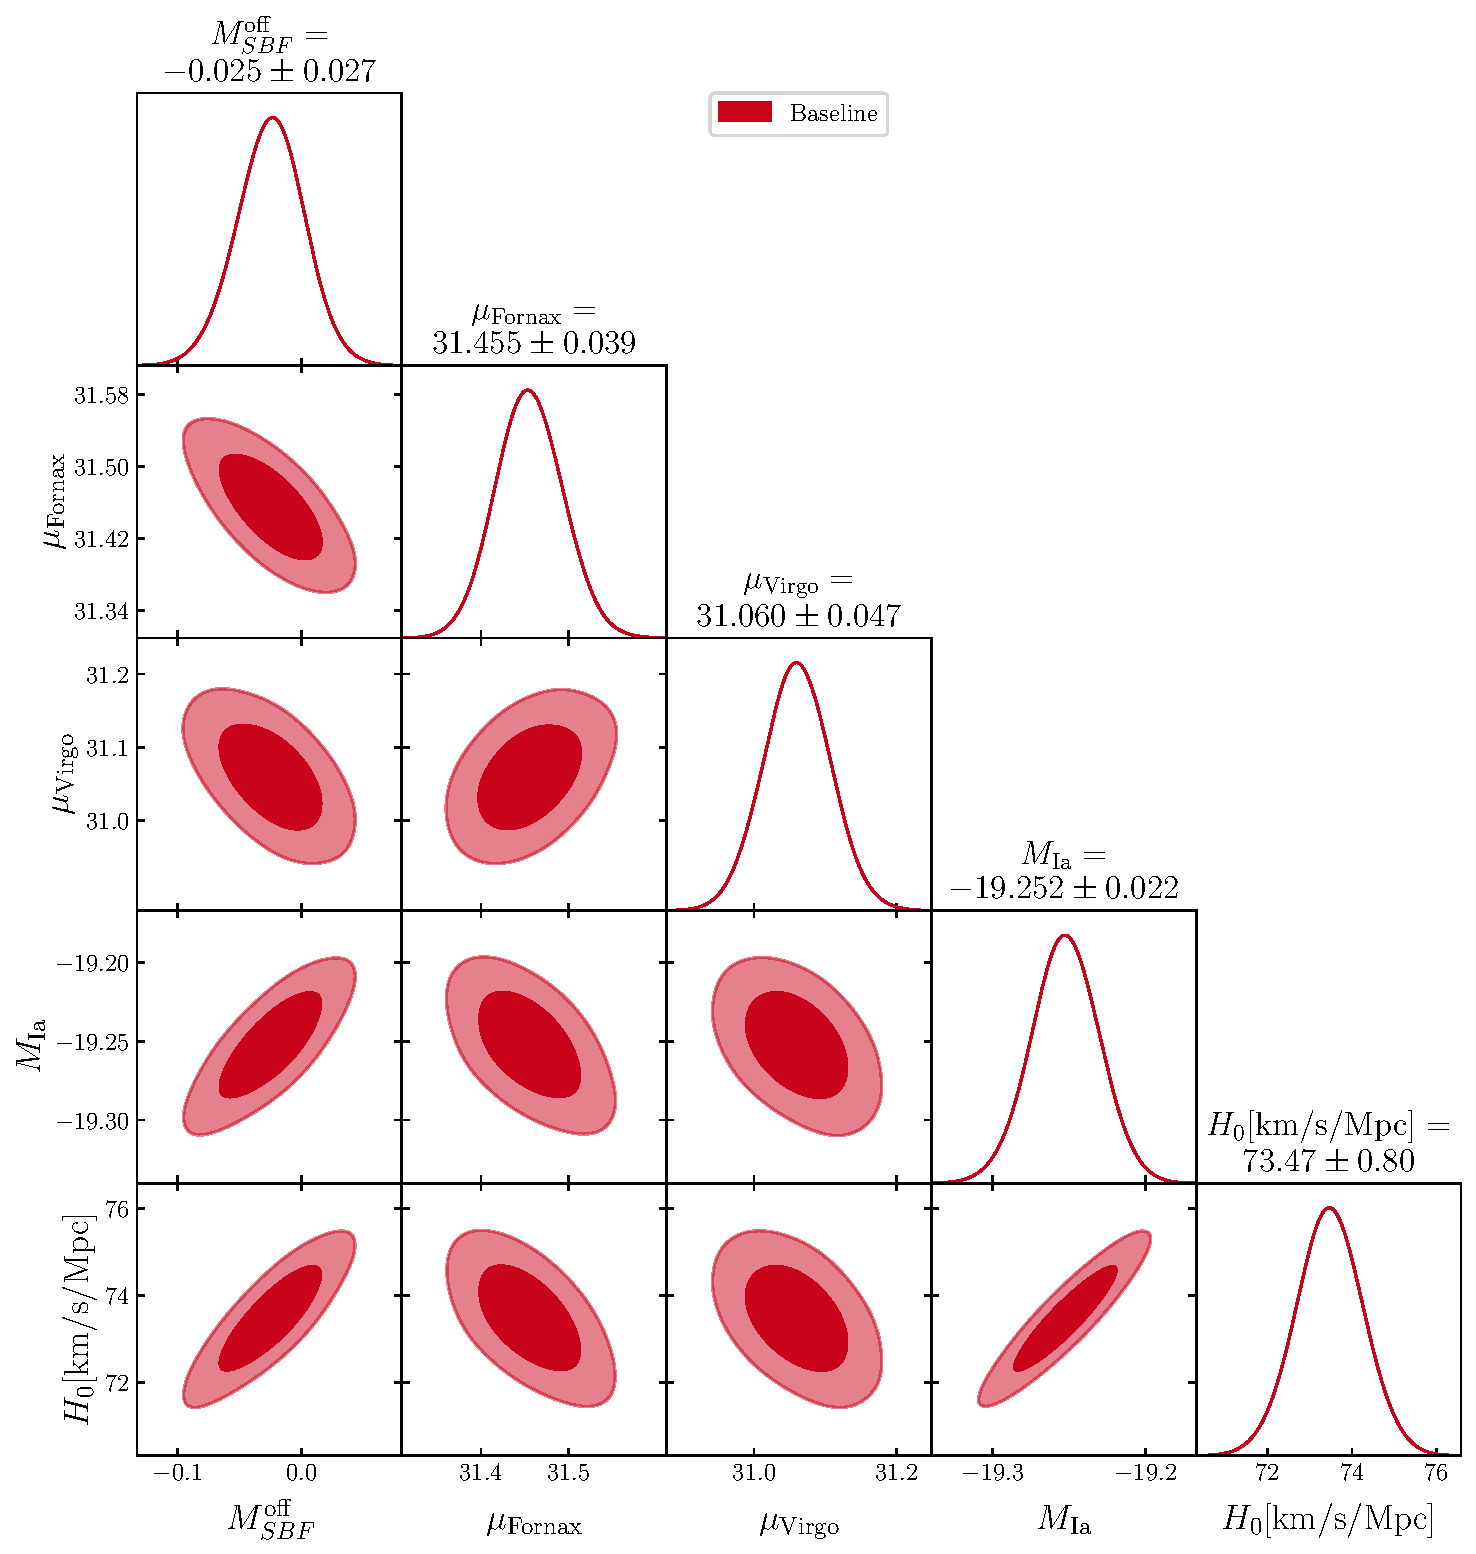
\includegraphics[width=0.9\linewidth]{Figures/chains_base_title_forpub.pdf}
    \caption{Corner plot for the baseline solution, illustrating the correlations between {\Hcst}, the calibration of SNe~Ia and SBF, and the distance to Fornax and Virgo, which contribute to the SBF calibration. The parameters use the naming convention of Appendix~\ref{sec:optimization_parameters}. Deviations from the analytically calculated result are due to the numerical precision of a finite-length chain.}
    \label{fig:baseline_corner}
\end{figure}

The solution for the baseline {\DN} yields the most accurate direct {\Hcst} measurement to date, with a relative uncertainty of \Hrelerrorbase, including systematic uncertainties. It agrees to much better than the $1\sigma$ uncertainty with previous determinations of {\Hcst} by the SH0ES team \citep{2022ApJ...934L...7R}.

The relative uncertainty of this result improves by  $\gtrsim 13\%$ over updates by the SH0ES team based on cluster Cepheids \citep{2022ApJ...938...36R} and sibling SNe~Ia \citep{2023JCAP...11..046M}, and by $\sim 7\%$ compared to the most recent SH0ES update provided by \citet{2024ApJ...973...30B}, which furthermore incorporated the SMC as an additional anchor. As shown by \citet{2022ApJ...934L...7R}, integrating TRGB distances into the fit strengthens the result, but does not cause it to deviate strongly. In the baseline case, this finding extends to the inclusion of distant megamasers and the SBF measurements. More generally, we find excellent agreement with most previous literature results based on direct measurements, as we show in Fig.~\ref{fig:whiskerCMB}---including most of the studies corresponding to the individual distance ladders that can be constructed within the {\DN}. We explicitly investigate the similarities and differences with respect to previous literature results that are part of the {\DN} in Appendix~\ref{sec:comparisons}, where we also showcase what is necessary to obtain the results with lower central values in \Hcst\,. We also find great agreement with the recent TDCOSMO results from \citet{2025arXiv250603023T}, which give $\Hcst = 71.6^{+3.9}_{-3.3}\Hunit$ and are compatible at $\sim0.5 \sigma$.

The consensus \Hcst{} measurement differs from the indirect, $\Lambda$CDM-dependent, measurement based on the CMB anisotropies of $\Hvaluecmb \pm \Herrorcmb \,\Hunit$ \citep[][Eq.~(54)]{2025arXiv250620707C} at a statistical significance of $\Hsigmabase \sigma$. 

\begin{figure}
    \centering
    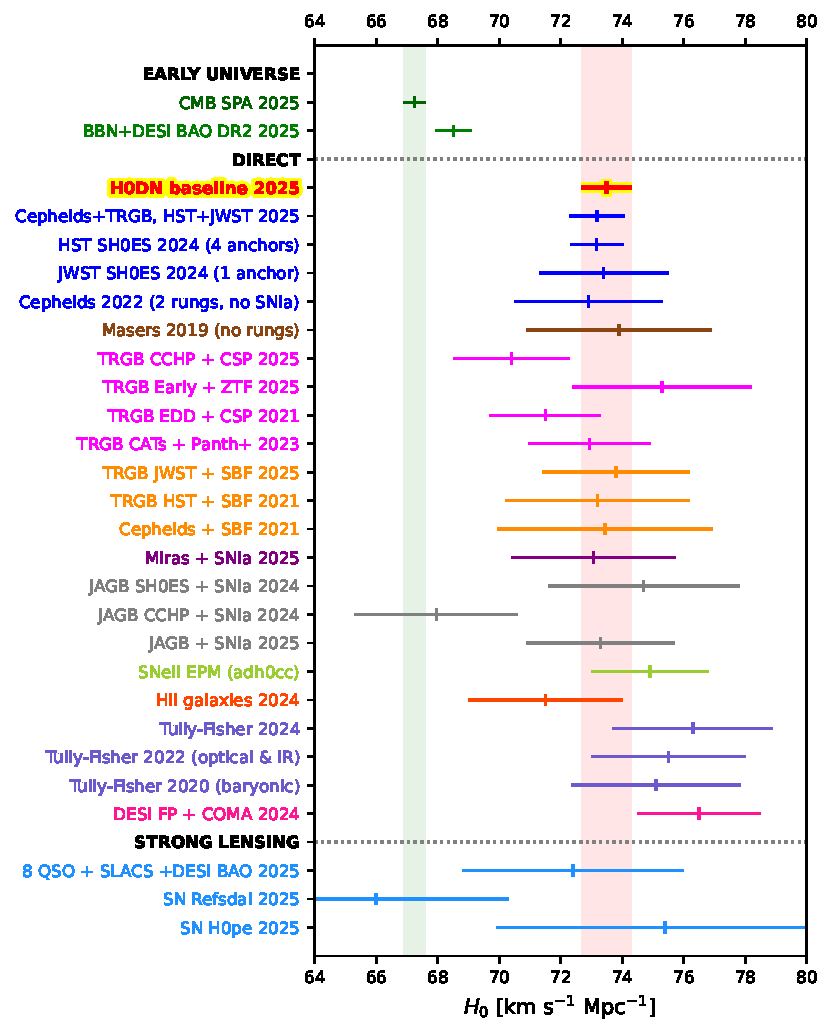
\includegraphics[width=0.8\linewidth]{Figures/H0_whisker_CMB.pdf}
    \caption{Comparison of the baseline result with  previous literature results, based on early universe indirect inferences using the flat $\Lambda$CDM model, based on direct measurements in the late universe, and based on strong lensing results (which involve additional modeling).
    }
    \label{fig:whiskerCMB}
\end{figure}


\section {Variants} \label{sec:variants}
Exploring variants to the baseline solution serves multiple purposes.  First, several available methods and data sets were not included in the baseline solution, for various reasons---primarily because of maturity of analysis or questions about uncertainty estimates. These data can still be used to highlight potential issues with the baseline solution, or point toward future research directions. In some cases, additional observations may eventually justify including these methods in the baseline. Second, it is informative to assess what happens to both the value and uncertainty in the Hubble constant when different categories of data are included or excluded in the solution. Third, some methods\hbox{---}e.g., SNe~Ia\hbox{---}can be included in several different ways; different filters, different light curve analysis, or different redshift selections. Finally, it is useful to consider a solution that includes all available, independent data and methods to assess the potential precision achievable with existing data once the remaining analysis issues are resolved. We stress that our process determined the baseline analysis as the primary solution \textit{priori to} obtaining any results on \Hcst{}. 
Variants in these categories are defined in Section~\ref{sec:variant_description}, and the results discussed in Section~\ref{sec:variant_results}.

Separately, we also consider two additional sets of consistency checks presented in Sect.\,\ref{sec:consistency_both}. One builds fully independent, ``orthogonal'' paths capable of determining \Hcst{} to verify that no single path/method dominates the \DN{}, cf. Section~\ref{sec:orthogonal_paths}.
The other employs a variety of different, albeit not independent, paths through the data to verify that their statistical properties are consistent with expectations, cf.~Section~\ref{sec:consistency_checks}. These checks serve to demonstrate the statistical consistency of the baseline solution with all possible configurations. Replications of results presented in the literature provide additional consistency checks of our methodology and are presented in Appendix~\ref{sec:comparisons}.


Some general considerations pertain to all these analyses and their interpretation. First, the baseline and variants were defined and classified {\it before} considering the resulting values of {\Hcst}. Very minor changes were introduced afterwards if required by updated data availability, albeit without changing the definition of the baseline.  
Second, most ``variants'' should not be regarded as alternative, equally valid solutions. Rather, their role is to illustrate the statistical properties of the data, identify potential problems, and/or reinforce their validity. This is especially true when considering the consistency checks, which are designed specifically so that each path uses only a small fraction of the available data, and thus has by construction a large nominal uncertainty, which is \textit{in no way} representative of the uncertainty in {\Hcst}. Third, the results of all variants are highly correlated because they share large portions of data. An exception are the orthogonal paths in Section~\ref{sec:orthogonal_paths}, which serve as consistency checks. Hence, the scatter between variants is expected to be much smaller than their error estimates. 

\subsection {Description of variants}\label{sec:variant_description}

The following is a short description of the main variants included in Table~\ref{tab:variants}. Specific sources of data products are provided in the text and in Appendix~\ref{sec:data_appendix}.

\begin{itemize}
\item[]\textbf{Baseline}
    \item[V00] Baseline: includes all measurements of SNe~Ia host distances using either Cepheids or TRGB, with the Milky Way via \gaia, the LMC, and NGC$\,$4258 as anchors, as well as SBF calibrated via TRGB and megamasers in the Hubble flow.   Note that TRGB distances are only anchored to NGC$\,$4258, since TRGB calibrations from the Milky Way and LMC do not meet our data requirements (notably photometric homogeneity across anchors and hosts in HST/JWST passbands).  Cepheids use all three anchors.  
    \smallskip\item[]\textbf{Add-one-in variants}
    \item[V01] Baseline + JAGB: includes all baseline methods, plus measurements of SNe~Ia hosts using the JAGB method, calibrated to NGC$\,$4258.
    \item[V02] Baseline + Miras: includes all baseline methods, plus measurements of SNe~Ia hosts using  Mira variables, calibrated to NGC$\,$4258.
    \item[V03] Baseline + Fundamental Plane: includes all baseline methods, plus distances to elliptical galaxies using the Fundamental Plane as measured by DESI, and calibrated to the distance of the Coma cluster measured with SBF and SNe~Ia.
    \item[V04] Baseline + empirically calibrated SNe II: includes all baseline methods and adds SNe~II (standard candle method) both as calibrators and in the Hubble Flow.  SNe~II host distances are determined via the distance network.
    \item[V05] Baseline + SNe~II with Expanding Photosphere Method: includes all baseline methods, plus SNe~II distances measured by the (astrophysical model-dependent) Expanding Photosphere Method.  Excludes a handful of supernovae that are too nearby to have significant weight on the determination of $ H_0 $.
    \item[V06] Baseline + Tully-Fisher: includes all baseline methods and adds calibrators for the Tully-Fisher relation and Tully-Fisher galaxies in the Hubble flow. The calibrators are treated in the same way as SNe Ia hosts, and their individual distances are determined from all available measurements.
    \item[V07] Baseline + SMC as anchor: includes all baseline methods and includes the SMC as an additional anchor for Cepheids.
    \smallskip\item[]\textbf{Leave-one-out variants}
    \item[V08] Baseline without Cepheids: excludes all Cepheid measurements from the distance network.  As a consequence, it only uses NGC$\,$4258 as anchor, since the Milky Way and LMC are currently only used via Cepheids. It furthermore excludes some SNe Ia for which TRGB measurements are not available.
    \item[V09] Baseline without TRGB: excludes all TRGB-based measurements.  As a consequence, it excludes some SNe Ia for which Cepheid measurements are not available, and the SBF method, which in this version it is only calibrated via TRGB.  A future version could include other primary distance indicators to calibrate the SBF method.
    \item[V10] Baseline without parallaxes: excludes parallaxes measured by {\it Gaia} and {HST}. As a consequence, the MW is removed as an anchor.
    \item[V11] Baseline without DEB distances to the LMC: removes the LMC as an anchor.  Note that the SMC is not included in the baseline.
    \item[V12] Baseline without NGC$\,$4258: this excludes all measurements based on NGC 4258 as anchor. As a consequence, all TRGB measurements are removed, since they are exclusively calibrated via NGC$\,$4258. As in V09, this also results in the exclusion of a number of SNe Ia for which no Cepheid measurements are available, as well as the SBF method.
    \item[V13]  Baseline without SNe~Ia: excludes all SNe~Ia, both as calibrators and as Hubble Flow objects.
    \item[V14]  Baseline without SBF: excludes all SBF-measured galaxies in the Hubble Flow.
    \item[V15]  Baseline without masers in the Hubble flow: retains the maser distance to NGC$\,$4258, but excludes other megamaser measurements. 
    \smallskip\item[]\textbf{Instrument-suspicious variants}
    \item[V16]  Exclude HST data: excludes {\it all} HST data from the baseline.  Since JWST anchor measurements are only available for NGC$\,$4258, this version also excludes the Milky Way and the LMC as anchors. 
    \item[V17]  Exclude JWST data: removes all JWST observations from the baseline.
    \item[V18]  Exclude SN~1994D and earlier: excludes 7 SNe~Ia calibrators that do not have modern data, namely SN 1980N, 1981B, 1981D, 1989B, 1990N, 1992A, and 1994D.
    \smallskip\item[]\textbf{Custom baselines}
    \item[V08B] Modified baseline for the no-Cepheid variant V08.  This is identical to the baseline, except that SNe~Ia for which we only have Cepheid distance estimates have been removed, leaving 35 SNe Ia calibrators.  Comparing V08 and V08B allows a direct estimate of the impact of removing Cepheids from the distance network, without the effect of changing the subset of SNe~Ia calibrators.
    \item[V09B] Modified baseline for the no-TRGB variant V09. This is identical to the baseline, except that SNe~Ia for which we only have TRGB distance estimates have been removed, leaving 42 SNe Ia calibrators. Comparing V09 and V09B allows a direct estimate of the impact of removing TRGB from the distance network, without the effect of changing the subset of SNe~Ia calibrators. However, this custom baseline includes SBF, which are excluded from V09 because they are calibrated using TRGB distances; therefore the difference between V09 and V09B is due to both the TRGB contribution to SN calibrator distances and to the omission of SBF.
    \item[V12B] Modified baseline for the no-NGC 4258 variant V12.  This is identical to the baseline, except that SNe~Ia for which we only have  distance estimates based on NGC 4258 have been removed, leaving 42 SNe Ia calibrators.  This variant allows a direct estimate of the impact of removing NGC 4258 from the distance network, without the effect of changing the subset of SNe~Ia calibrators.  Unlike V09B, this custom baseline also excludes SBF measurements;
    therefore the difference between V12 and V12B is only in the contribution of NGC 4258 to the distances to SNe Ia calibrators.  
    \item[V16B] Modified baseline for the no-HST variant V16. This is identical to the baseline, except that SNe~Ia for which we only have HST-based distance estimates have been removed, leaving 24 SNe Ia calibrators. Comparing V16 and V16B allows a direct estimate of the impact of removing HST measurements from the distance network, without the effect of changing the subset of SNe~Ia calibrators.
    \smallskip\item[]\textbf{Hypothesis-driven variants} 
    \item[V19] Modified baseline in the CMB frame: removes the peculiar velocity corrections for SNe~Ia, SBF, and megamasers in the Hubble flow.
    \item[V20] Modified baseline that limits Hubble flow SNe~Ia to $ 0.023 \leq z \leq 0.06 $.
    \item[V21] Modified baseline, with SNeIa in the Hubble flow limited to $ 0.03 \leq z \leq 0.1 $.
    \item[V22] Modified baseline, with SNeIa restricted to the CSP sample fit using SNooPy v2.7 for both calibrators and tracers. 
    \item[V23] Modified baseline with SNe~Ia measurements fitted using BayesSN for both calibrators and Hubble flow objects.
    \item[V24] Modified baseline, wherein SNe\,Ia light curves were fitted using the SALT V3 fitter instead of SALT V2.4 (as in Pantheon+)
    \item[V25] Modified baseline that exclusively uses H-band NIR measurements for both calibrators and Hubble flow SNe~Ia.
    \item[V26] Modified baseline that exclusively uses J-band NIR measurements for both calibrators and Hubble flow SNe~Ia.
    \item[V27] Modified baseline that ignores off-diagonal covariance terms for Hubble flow SNe~Ia.
    \item[V28] Modified baseline without metallicity corrections for Cepheid PL relation
    \smallskip\item[]\textbf{Include everything}
    \item[V99] ``Everything'': All data included in any variant, without repeating Hubble Flow objects; SNe~Ia exclusively from Pantheon+.
   \item[V99a] ``Everything but Tully-Fisher'': as V99, but excludes the Tully-Fisher method, which contributes to the total $ \chi^2 $ beyond expectations, and has high $ \chi^2 $ in the Hubble Flow.
\end{itemize}

\input Tables/vartable.tex

\begin{figure}
    \centering
    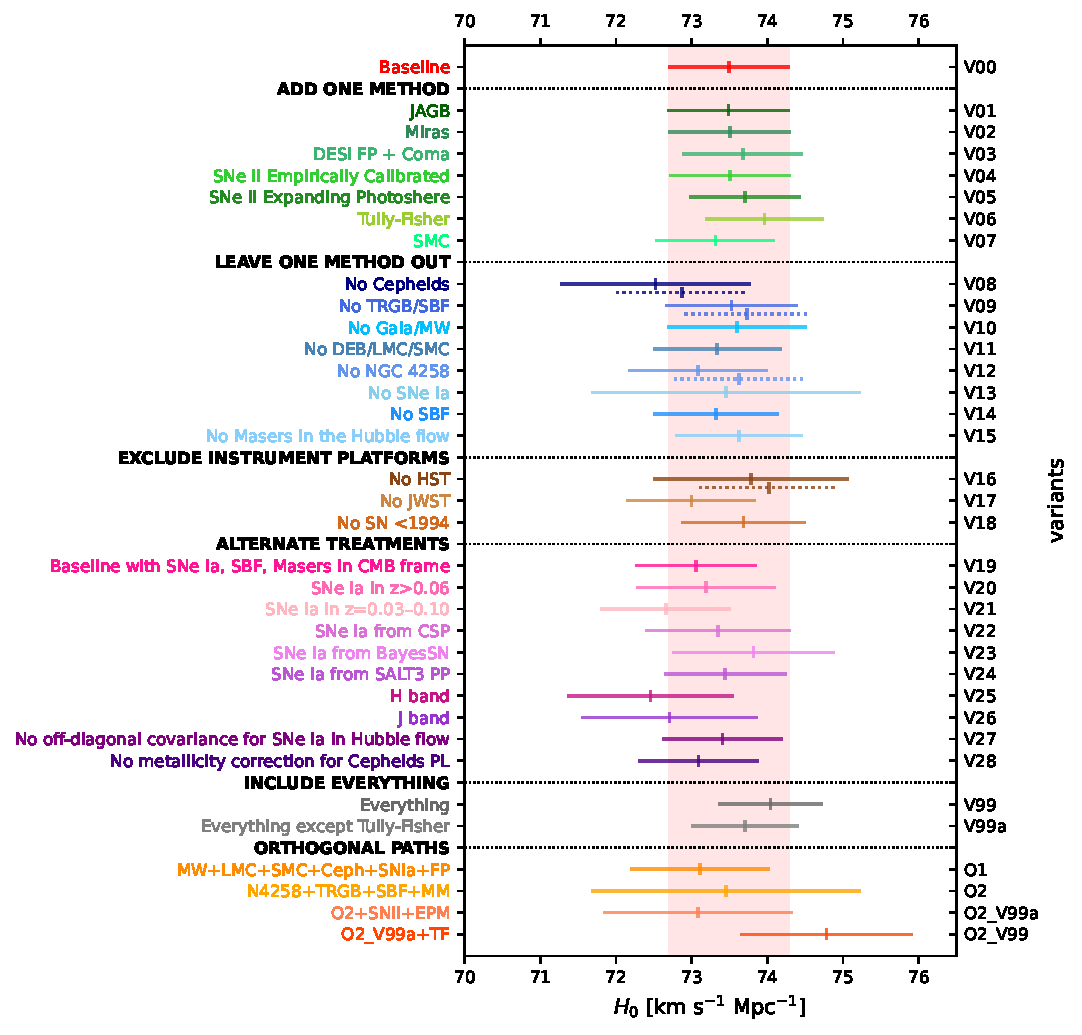
\includegraphics[width=\linewidth]{Figures/H0_whisker_solid.pdf}
    \caption{Baseline and variants results from Table~\ref{tab:variants}. For some variants, a labeled change has a secondary consequence (i.e., removing the identified primary distance indicator also results in the loss of calibration to some SN Ia).  In these cases a dashed line immediately below such variants provides a custom baseline--i.e., the same SNe are removed before the removal of the primary indicator--is shown to provide a custom reference of impact for that variant; see text for details.
    }
    \label{fig:whisker}
\end{figure}

\subsection{Overview of results based on variants} \label{sec:variant_results}

The results of the baseline and all variants are illustrated in Figure\ref{fig:whisker} and reported in Table~\ref{tab:variants}. All variants yield results consistent with the baseline, typically varying only slightly from the baseline result; the dispersion of central values is $0.400$\,\Hunit, or $50\%$ of the baseline's $1\sigma$ uncertainty. Since the baseline and its variants are highly correlated due to shared datasets and methodologies, a scatter significantly below $1\sigma$ is expected. The absence of outliers among the variants demonstrates that the results are not driven in any particular direction by any one dataset or methodology, or any of the hypothetical systematics explored. For example, variants V08, V10, and V13 demonstrate that the central value of {\Hcst} is not dominated by Cepheids (V08), parallaxes mainly from {\it Gaia} (V10), or SNe~Ia (V13).  
Figure~\ref{fig:whisker} also readily identifies differences in constraining power brought by various methods: the largest increases in the error on \Hcst{} are seen in V08 (no Cepheids), V13 (no SNe\,Ia), and V16 (no HST). This underlines the crucial precision provided by Cepheids, SNe\,Ia, and {HST} observations, whereas the insensitivity of the central value on \Hcst{} demonstrates that neither dominate the result.
The exploration of such variants establishes robustness of the baseline result and demonstrates that the {\DN} is enhanced by the joint consideration of complementary methodologies. It further underlines that the different methodologies reinforce and strengthen each other, resulting in improved accuracy thanks to the DN approach.  

\subsubsection {Adding one class at a time}

Variants V01 to V07 each add one category of objects or methodology to the baseline solution; these include JAGB, Miras, the Fundamental Plane of elliptical galaxies, empirically and astrophysically calibrated SNe~II, Tully-Fisher, and the SMC as an additional anchor.  For all cases except the Tully-Fisher relation, the impact on the solution is negligible, with the central value of $ H_0 $ changing by 0.2 {\Hunit} or less ($25\%$ of the $1\sigma$ uncertainty), and the uncertainty remaining constant or decreasing slightly.  Including astrophysically calibrated SNe~II (V05) leads to the most significant improvement to the uncertainty, by $8.5\%$ to $ \Herrorepm \Hunit $; however, this method being relatively new, its systematic uncertainties are not yet fully quantified \citep{2025AA...702A..41V}.  

Including the Tully-Fisher relation raises $ H_0 $ by almost 0.5 {\Hunit} ($\sim 60\%$ of the baseline error), and yields a reduced $ \chi^2 $ significantly larger than unity (\redchisqtf). The increase in $ H_0 $ is consistent with the results of the recalibration of the Tully-Fisher relation by \cite{2024arXiv241208449S}.  Inspection of the residuals shows that the anomalous value of $ \chi^2 $ is caused by the dispersion in predicted magnitude for Tully-Fisher calibrators, whose empirical scatter significantly exceeds the assumed intrinsic dispersion, particularly at the bright end. Uncertainties in host distances are subdominant and unlikely to play a role in this comparison. We conclude that the internal dispersion currently assumed for the Tully-Fisher relation is likely underestimated, and recommend avoiding the inclusion of Tully-Fisher results until its intrinsic dispersion can be reevaluated.

 \subsubsection {Leave-one-out variants\label{sec:leave-one-out}}

Variants V08-V18 each remove one class of measurements or a subset of data from the solution.  Most variants do not change the central value of {\Hcst} much, with the exception of V08 (no Cepheids), which drops it by almost 1 {\Hunit} to {\Hvaluenoceph} {\Hunit}, and V12 (no NGC 4258), which decreases it to {\Hvaluenoftfe} {\Hunit}. 
Comparing V08 and the corresponding custom baseline (V08B) clearly identifies that the shift in the no-Cepheids variant (V08) is driven by the implicit exclusion of 20 calibrator SNe\,Ia rather than by the Cepheids themselves. Analogous effects on \Hcst{} induced by subsampling SNe\,Ia calibrators have been extensively discussed in \citet{2024ApJ...977..120R}. Accounting for this effect leaves a difference of merely $0.352$\,\Hunit\ ($44\%$ of the baseline error) due to excluding Cepheids.

Some variants yield significantly increased uncertainties on \Hcst{}. Excluding Cepheids (V08) increases the uncertainty from {\Herrorbase} to {\Herrornoceph} {\Hunit}, and comparison with the uncertainty of the custom baseline V08B (\Herrorcustbasenoceph) reveals that this increase is truly driven by the exclusion of Cepheids rather than the implicitly removed 20 SNe\,Ia calibrators. 
More modest increases occur for the variants without NGC$\,$4258 as anchor, or when TRGB measurements are excluded. This is simply a reflection of the reduced constraining power caused by the exclusion of a broad class of measurements. Excluding either the Milky Way or the LMC as anchors has less impact, as each exclusion leaves two anchors for Cepheids, and does not affect the TRGB, which is only calibrated via NGC$\,$4258. The most dramatic impact is associated with the exclusion of all SNe~Ia; this increases the uncertainty to {\Herrornosnia} {\Hunit}, more than a factor of 2 above the baseline, illustrating the strong constraining power of SNe~Ia, which remain the most powerful way to measure the local value of the Hubble constant. 
When SNe Ia are excluded from the baseline, the primary constraint on {\Hcst} is based on the SBF measurement. Even in this case, the central value of {\Hcst} is changed only little, although one naturally finds a much larger uncertainty. As an illustration, the solution including all other available data but excluding SNe~Ia in the Hubble flow---formally not a variant, since it does not satisfy the criteria established during the Workshop---yields $ \Hvaluehfnosnia \pm \Herrorhfnosnia \, \Hunit $; despite the higher uncertainty, this value is still $\Hsigmahfnosnia \, \sigma $ away from the CMB value in flat $\Lambda$CDM.

The two variants V16 and V17 explore the impact of excluding all calibrator  data from either HST or JWST, testing potential broad systematics, such as calibration errors, that affect either facility. Note that all primary distance indicators as included used space-based data from at least one of the two facilities.
Excluding HST also implies excluding the Milky Way and the LMC as anchors, since we do not yet have a calibration for Cepheids in those systems based on JWST data.  The solutions with either no HST or no JWST data are not fully disjoint since they share a common anchor, NGC 4258, and many of the Hubble Flow tracers, and since the set of calibrators overlap, carrying with them any intrinsic variance in their properties.  However, many of the sources of uncertainty in distance estimates are different and independent. The resulting {\Hcst} values bracket the baseline, as could be expected, with a difference in line with their respective uncertainties: without HST, $ \Hvaluenohst \pm \Herrornohst \, \Hunit $; and without JWST, $ \Hvaluenojwst \pm \Herrornojwst \, \Hunit $.  Not surprisingly, the uncertainty in the result increases more if HST is excluded, since HST results use three anchors (only NGC 4258 is available for JWST) and more HST observations are available, yet both subsets remain close to the baseline with a difference below $ 1 \, \Hunit $. The fact that the inclusion of JWST observations favors a higher value of \Hcst{} corroborates the conclusion based on host-to-host distance comparisons by \citet{2024ApJ...977..120R} that \Hcst{} measurements based purely on HST \citep{2022ApJ...934L...7R} are not biased high by the limited spatial resolution of WFC3/IR (crowding).

\subsubsection {Alternate treatments\label{sec:alternative_medicine}}

Variants V19-V26 show what happens if subsets of data are either excluded or treated differently. For variants V19-V22, we modify the handling of peculiar velocities or redshift selection. In variant V19, we assume that the observed velocities directly represent cosmological redshifts, i.e., we set all peculiar velocity corrections, which are by default derived with the 2M++ model \citep{2015MNRAS.450..317C}, to zero.  The value of {\Hcst} decreases slightly, to $ {\Hvalueusecmb} \pm {\Herrorusecmb} \, \Hunit $, with no meaningful change in the accuracy.
Similarly, restricting the redshift range, either by removing the high redshift end (V20, $ z > 0.06 $) or the low-redshift end (V21, $ 0.3 < z < 1 $), changes the value of {\Hcst} by up to 0.8\,{\Hunit}; the impact on the accuracy is modest.

Variants V22-V27 are noteworthy because they explore different treatments of SNe\,Ia, which drive overall precision (cf. Sect.\,\ref{sec:leave-one-out}). 
Variants V22 and V23 consider different light curve fitters (consistently for both calibrators and tracers), namely SNooPy v2.7 in V22 and BayesSN in V23. Both variants yield slightly higher \Hcst{} values with slightly larger nominal uncertainties. The BayesSN variant V23 furthermore yields a higher reduced $ \chi^2 $. Further detail and comparisons with published articles is provided in App.\,\ref{app:sec:SNIa_literature}, specifically concerning SNooPy in App.\,\ref{app:snoopy}.

Variants V25 and V26 rely exclusively on NIR measurements for SNe~Ia \citep{2023AA...679A..95G}, in the $ H $ and $ J $ band respectively. These also yield slightly lower, yet consistent \Hcst{} results with slightly larger uncertainties due to the smaller number of calibrators and Hubble flow tracers.  Note that we did \textit{not} use SNe~Ia measurements from multiple sources (e.g., Pantheon+ and NIR) simultaneously in any solution; doing so would lead to unreliable, likely incorrect results.  First, the calibration of SN measurements in different samples are inconsistent, as they are based on different filters, fitting processes, and conventions.  More importantly, different measurements of the same SN would share to a large extent the astrophysical variance of the source; therefore we expect such measurements to be significantly correlated in their deviation from the mean, to an extent that; to the best of our knowlegde, has not been sufficiently quantified.  Since the SNe~Ia samples overlap significantly, multiple measurements cannot be included in the same solution in a statistically satisfactory way.  To avoid such issues, we take care not to include multiple measurements of the same SNe~Ia---whether as local calibrators or as Hubble flow objects---in the same solution. Unless otherwise stated, all solutions exclusively consider measurements collected in the Pantheon+ system \citep{2022ApJ...938..113S}.

Another treatment option concerns the covariance between different SNe~Ia in the Hubble flow. Several collections of measurements provide covariances between different objects; these can be due to the effect of standardization parameters, or the survey from which data have been obtained. By default, we include such covariances where available. However, Variant V27 deliberately ignores these covariances and assumes (incorrectly) the stated uncertainties to be independent in order to assess the impact that the SNe\,Ia covariances have on the final result. This results in a miniscule decrease in {\Hcst}, by less than 0.1\,{\Hunit}, and analogously miniscule decrease in the nominal uncertainty. We conclude that covariances between SNe~Ia measurements in the Hubble flow currently have a negligible impact on \Hcst. 

\subsubsection {``Everything'' solution\label{sec:everything_bagel}}

It is naturally interesting to consider the result of including all available methods into the \DN{}. To this end, we constructed variant V99 by including all available measurements.
As noted above, multiple measurements of SNe~Ia cannot be combined in a statistically satisfactory way, so that V99 exclusively considered Pantheon+ SNeIa. V99 also incorporates methods with as yet insufficiently well understood systematics, such as SN~II with EPM and the Tully-Fisher relation. 
These results are provided here for completeness, and we recommend that they \textit{not} be used for further analysis.  The resulting value is $ \Hvalueeverything \pm \Herroreverything \, \Hunit $, which lies $ \Hsigmaeverything \, \sigma $ from the Planck+$\Lambda$CDM solution.  We recognize that this solution may not be fully reliable, as indicated by the relatively large value of reduced $ \chi^2 $, namely $\redchisqeverything $ per degree of freedom; indeed, this solution deviates from the baseline more than several others, primarily because of the TF contribution.  Since the TF relation contributes the most to the excess $\chi^2 $, we also include variant V99a, which is identical to V99 except for the exclusion of TF calibrators and tracers.  This variant results in $ \Hcst = \Hvalueeverythingnotf \pm \Herroreverythingnotf \Hunit $, very close to the baseline with a 12\% smaller uncertainty (and sub-percent precision on \Hcst), has a reasonable reduced $ \chi^2 $ of {\redchisqeverythingnotf}, and lies $ \Hsigmaeverythingnotf \, \sigma $ from the Plank+$\Lambda$CDM solution. 

The everything solution is useful to understanding how elements in the baseline solution compare to the elements not included therein, as well as any covariances among them. Three figures illustrate these points. Figure\,\ref{fig:everything_residuals} shows the fit residuals of host and calibrator distances for V99 in analogy with Fig.\,\ref{fig:baseline_residuals} for the baseline. Figure\,\ref{fig:everything_hf} illustrates the corresponding Hubble flow residuals for V99. A corner plot illustrating covariance among the main global fit parameters of the \DN{} for V99 is shown in Fig.\,\ref{fig:everything_corner}. 

\begin{figure*}
    \centering
    \includegraphics[width=0.9\linewidth]{Figures/ISSI-H0-Workshop-DistanceNetwork-all-batlowKS.pdf}
    \caption{Residuals for host and calibrator distances for the ``everything'' solution.  The groupings, also distinguished by color, correspond to calibrators measured by the same authors with common method and anchor.  The error bars reflect the individual calibrator errors; the shaded areas for each group indicate the combined uncertainty in the anchor distance and its reference value, which are in common for all calibrators in the same grouping.}
    \label{fig:everything_residuals}
\end{figure*}

\begin{figure*}
    \centering
    \includegraphics[width=0.9\linewidth]{Figures/ISSI-H0-Workshop-HubbleFlow-all-batlow25-Log.pdf}
    \caption{Residuals in $ \log(H_0) $ vs.\ redshift for objects in the Hubble Flow for the ``everything'' solution.  Each subplot refers to sources in the same group, measured by the same method.  Error bars for individual sources are representative of the expected scatter across sources in the same category, and do not include calibration uncertainties for each class.  The shaded bars at the right show the mean and dispersion for each category.}
    \label{fig:everything_hf}
\end{figure*}

\begin{figure}
    \centering
    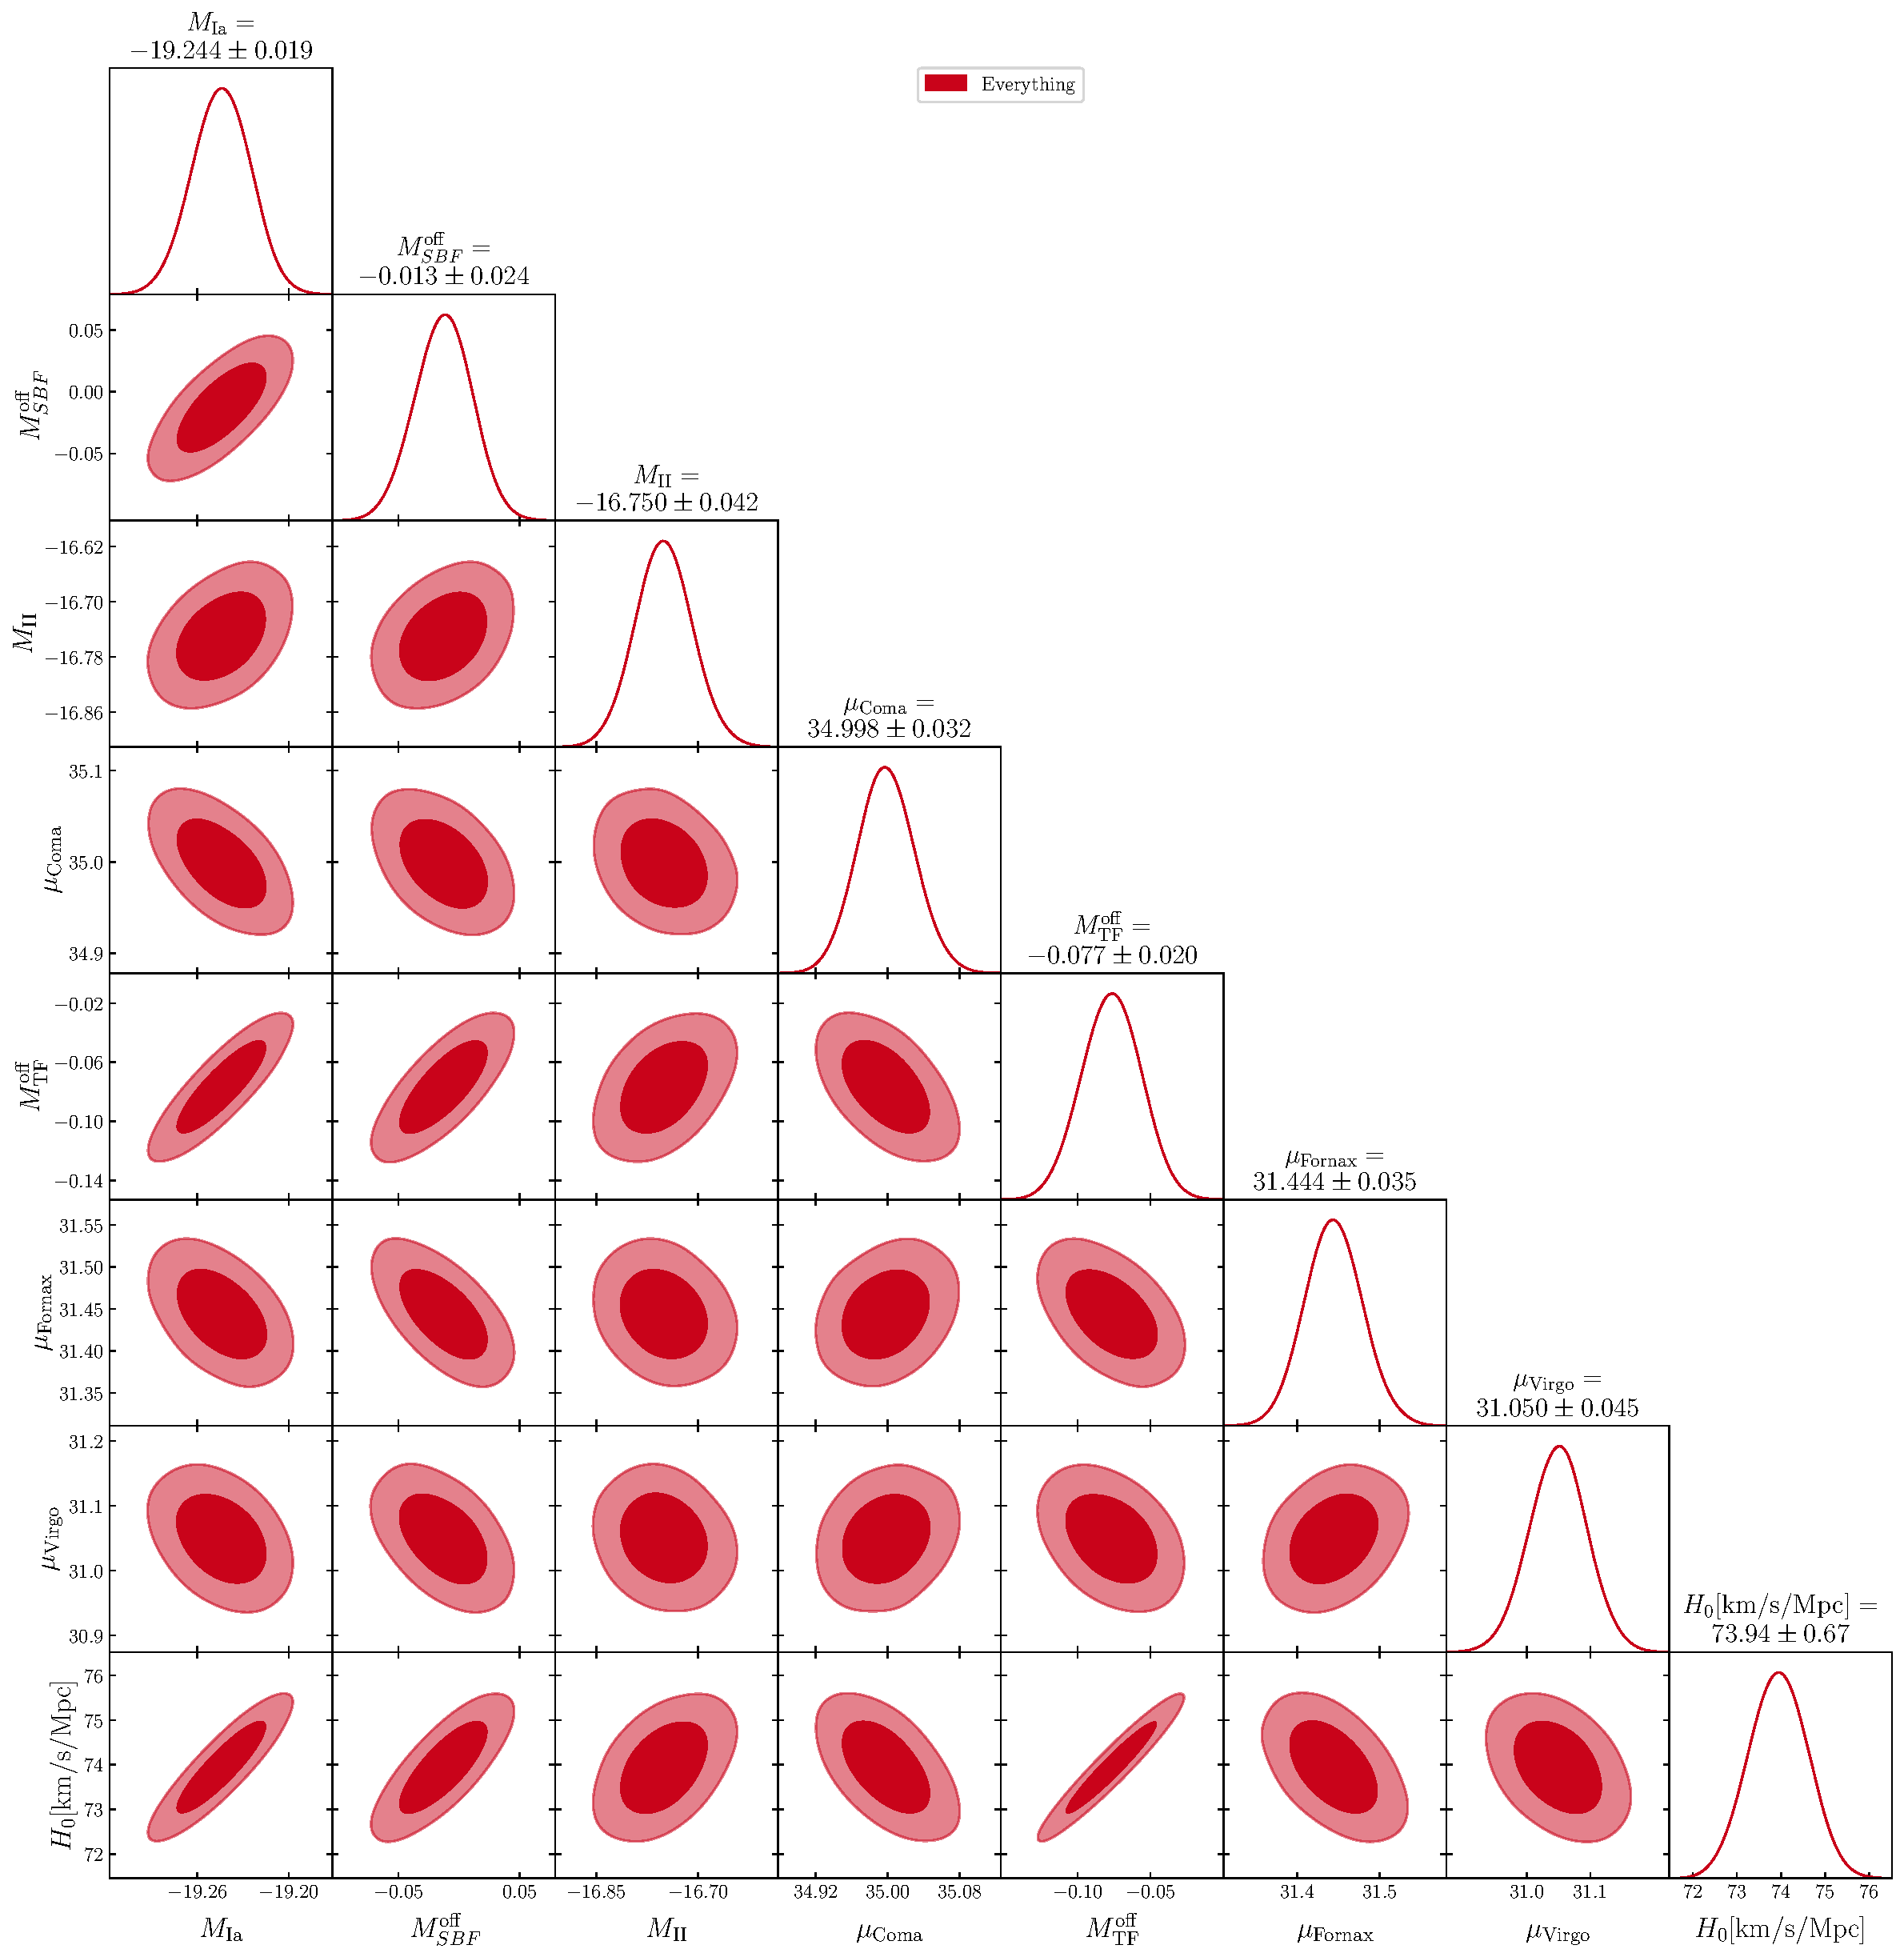
\includegraphics[width=0.9\linewidth]{Figures/chains_all_title_forpub.pdf}
    \caption{Corner plot illustrating the main optimization parameters for the all-inclusive solution, using the naming convention of Appendix~\ref{sec:optimization_parameters}.  Parameters related to individual host distances are not included. Note that this solution is not an alternative result to the baseline solution, but rather a variant to check the impact of further data on our result, see also Section~\ref{sec:variants}. We show it here to highlight the existing correlations between the various (most important) solution parameters. Deviations from the analytically calculated result are due to the numerical precision of a finite-length chain.}
    \label{fig:everything_corner}
\end{figure}

\subsection{Consistency Checks\label{sec:consistency_both}}
We demonstrated the statistical consistency of the baseline solution by building alternate paths through the \DN{} capable of determining \Hcst{}. Statistically independent paths are discussed in Sect.\,\ref{sec:orthogonal_paths}, statistically not independent paths in Sect.\,\ref{sec:consistency_checks}. Replications of \Hcst{} results from the literature are presented in Appendix~\ref{sec:comparisons}.

\subsubsection{Orthogonal paths}\label{sec:orthogonal_paths}

Orthogonal paths strike statistically fully independent paths across the \DN{}. In creating these paths, we sought to identify configurations capable of achieving similar constraining power.
We identified the following two\footnote{In principle, more orthogonal paths could be formulated (e.g., by separating out specific one-step methods), but such combinations of paths are typically not balanced in their constraining power.} orthogonal paths and two extensions of the latter:
\begin{itemize}
    \item \textbf{O1:(MW+LMC+SMC+Ceph+SNIa+FP)} employs the Magellanic Clouds and MW parallaxes as anchors, calibrates SNeIa using Cepheids, and adds in the FP calibrated in Coma. This yields $\Hcst = 73.11 \pm 0.92 \Hunit$ with a $\chi^2=53.5$ and a reduced $\chi^2$ of 0.922.
    \item \textbf{O2:(N4258+TRGB+SBF+MM)} Uses N4258 as anchor, TRGB as calibrators, and SBF as tracers, in addition to megamasers. This corresponds to a modified V07 (baseline+SMC) from which all measurements correlated with O1 have been removed. This yields $\Hcst = 73.45 \pm 1.78 \Hunit$, with a $\chi^2=11.2$, and a reduced  $\chi^2$ of 0.4853. The low reduced $\chi^2$ indicates that the measurement uncertainties used are overestimated.
    \item \textbf{O2\_V99a:(O2+SNII+EPM)} Modified O2 to which both astrophysically and empirically calibrated SNe\,II have been added, i.e., corresponds to V99a without elements in O1. We find $\Hcst = 74.06 \pm 1.25 \Hunit$, with a $\chi^2=28.76$, and a reduced  $\chi^2$ of 0.5752. Here too the reduced $\chi^2$ is a little low.
    \item \textbf{O2\_V99:(O2\_V99a+TF)} Modified O2 with Tully-Fisher relation added, i.e., corresponds to V99 without the elements in O1. We find $\Hcst = 74.93 \pm 1.14 \Hunit$, with a $\chi^2=186.6631$, and a reduced  $\chi^2$ of 1.4359. The very significant increase in reduced $\chi^2$ emphasizes the underestimated uncertainties of the Tully-Fisher results, cf. V99.
\end{itemize} 
Fig.\,\ref{fig:paths_orth} illustrates the results of these orthogonal paths compared to the baseline result. Both O1 and O2 are highly compatible with each other, deviating by only $0.17\sigma$ despite representing fully independent measurements. As previously shown in the context of V13, the significantly higher uncertainty of O2 is due to the exclusion of SNe\,Ia. 
The orthogonal nature of O1 and O2 allows to compute their weighted average, $H_0^\mathrm{O1+O2} = (73.18\pm 0.82)\Hunit$, which agrees to within $0.3\,$\Hunit{} of the baseline. The slightly offset central value and reduced precision arise due to fewer internal cross-calibrations---their combination is missing for example any N4258-anchored calibrations of SNe~Ia. This underlines a key advantage of the covariance-combined approach taken by the H0DN collaboration compared to independent pursuits of \Hcst{}\,.

The two extensions to O2 considered, O2\_V99a and VO2\_V99, add elements from the ``everything'' variants (V99a, V99) to improve precision. Both extensions yield \Hcst{} values marginally higher than O2 and fully compatible with the respective ``everything'' variants V99 and V99a. The weighted average $H_0^\mathrm{O1+O2\_V99a} = (73.45\pm 0.74)\Hunit$ agrees to within $< 0.5\sigma$ with V99a and features a very similar uncertainty. Finally, the weighted average including the Tully-Fisher relation, $H_0^\mathrm{O1+O2\_V99} = (73.77\pm 0.71)\Hunit$, agrees to within $0.4$\,\Hunit{} with V99, with also very similar uncertainty.

Overall these tests confirm both the reliability of the main results as well as the consistent setup of the network. We note that in the case in which the baseline is split into two orthogonal paths we have a mild domination of the uncertainty by the SNe~Ia, whereas in the extended cases the uncertainties are relatively balanced.

\subsubsection{Paths based on subsets of data} \label{sec:consistency_checks}

In order to verify the internal consistency of different data sets and methods relevant to determining the Hubble constant, 
we show below the $H_0$ values obtained for a set of ``paths'' through the network, each defined by a unique combination of anchors, calibrators, and tracers.\footnote{In practice we construct these paths as minimal combinations, except where this might lead to ambiguities. First we use each of the possible calibrator sets (e.g. Cepheids measured with HST, or Miras, or JAGB, etc.) together with the SNe~Ia as Hubble flow tracers (13 combinations), then using the SNe~II (either just with the minimal calibrator set from \citet{2020MNRAS.496.3402D} or with all available calibrators) (2 combinations), the megamasers alone, the SBF anchored using any hosts anchored by NGC$\,$4258, and the SNII tailored~EPM method (each 1 path), as well as the FP method anchored only by the SBF value (to remain minimal). In total that makes 19 paths through the network.} These paths are not all statistically independent by definition, since they might share, for example, a common anchor or a common set of tracer objects. However, we expect the corresponding distribution of $H_0$ values to align at least as well as for independent variables, since we expect the shared data to produce positive, not negative, correlations. In this case, the corresponding test statistics can be regarded as lower bounds on the true values that would be obtained if the full correlation structure were accounted for (i.e., in plain English: ``if the points sharing the same data are incompatible, that's even worse than points not sharing the same data being incompatible''). We find that the Anderson-Darling test \textit{cannot} reject the null hypothesis of the paths stemming from a Gaussian distribution at 5\% confidence level, and we find $p=86.3\%$ for the Shapiro test, both very well within acceptable bounds. We also find no visually strong $(>2\sigma)$ outliers among the paths shown in Figure~\ref{fig:paths_consistency}. Note that since these paths are constructed always using minimal paths through the network, they explicitly do not qualify as `variants' in the sense defined above. We also note that if we were to include the Tully-Fisher case in the generation of these paths, the results worsen quite a bit, to a $p \simeq 10\%$ for the Anderson-Darling test and a $p\simeq 5\%$ for the Shapiro test, showing once again the high discrepancy of the Tully-Fisher based results within the {\DN}.

\begin{figure}
    \centering
    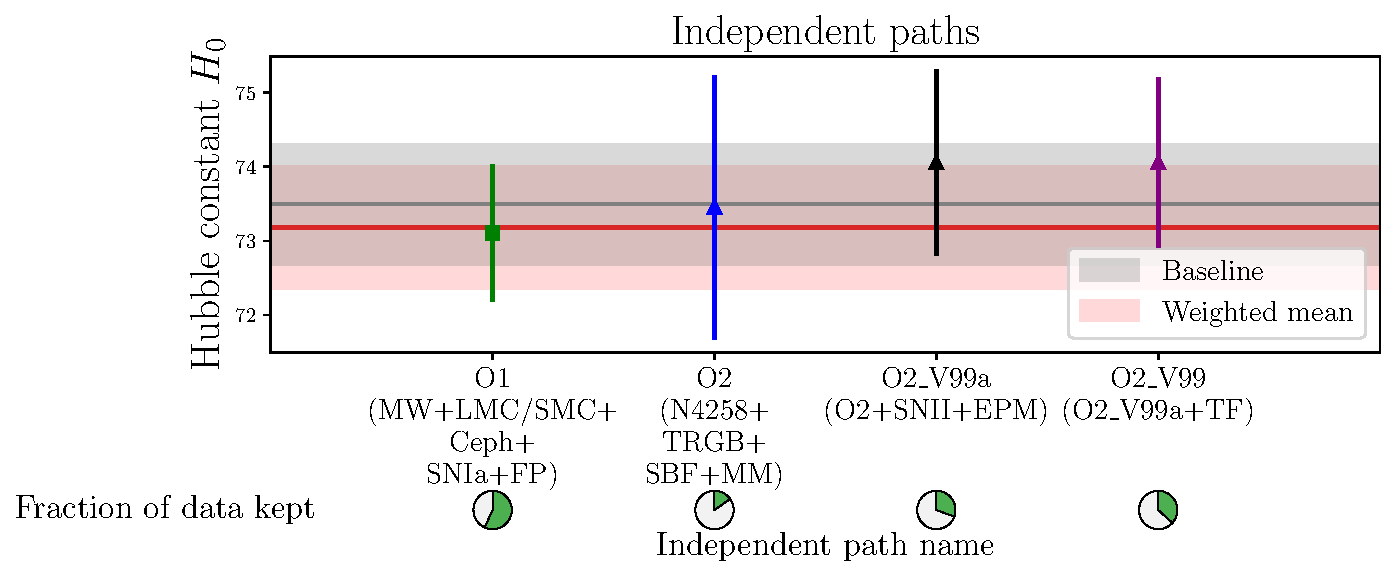
\includegraphics[width=0.79\linewidth]{Figures/o_paths_v3.pdf}
    \caption{The two paths starting with ``O'' are proper orthogonal paths and can be taken as independent measurements of the Hubble constant. Their weighted mean (red) agrees well with our baseline result despite the latter including all cross-correlations. The shortcuts of the data sets are as defined in the text. The pie charts  ``fraction of data kept'' represent the fraction of statistical power remaining in the path. It is computed as the fraction of the variance of {\Hcst} for the given result (in this way multiple datasets with the same constraining power in $H_0$ will be assigned equal percentages). We show the percentages relative to the baseline result (V00).}
    \label{fig:paths_orth}
\end{figure}

\begin{figure}
    \centering
    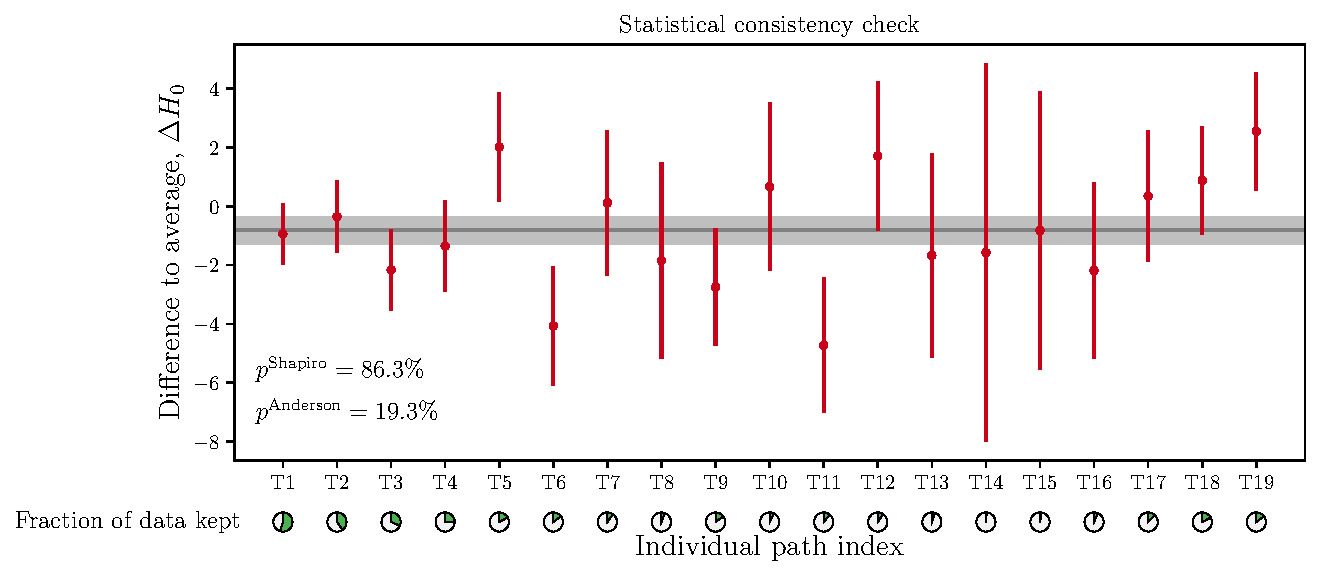
\includegraphics[width=0.79\linewidth]{Figures/paths_v6.pdf} 
    \caption{The statistical consistency of various individual paths through the network. These represent a set of paths that are highly correlated, and often only take a tiny part of the network into account. They are used for a statistical consistency check and should not be interpreted as valid variants in the sense of section \ref{sec:select_variants}. We also show the simple weighted mean of these paths in grey purely for visual purposes, reminding that due to their correlations (and selection effects) it need not necessarily agree with the baseline result. For details on the pie charts, see Fig.~\ref{fig:paths_orth}.}
    \label{fig:paths_consistency}
\end{figure}


\section{Conclusions and Discussion} \label{sec:conc}
The Hubble ``tension'' has persisted for more than a decade and significantly shifted focus amongst endeavors to precisely measure \Hcst. Before $\sim$2012, the primary motivation for measuring $H_0$ with increasing precision was to provide a strong prior for constraining $\Lambda$CDM parameters and understanding dark energy \citep[e.g.,][]{Suyu:2012}. As the statistical significance of the discrepancy between early- and late-Universe measurements grew, relentless attention was given to systematics of local distance measurements with an implicit expectation that the tension would be resolved once the responsible systematic error was identified. In other words, there was a non-negligible preference among many to discard direct measurements (even ones with small and detailed uncertainties) based on astronomical techniques in favor of the \Hcst\ value derived from the perceived ``simple physics'' of the early Universe and a specific cosmological model. A narrative of merely two or three direct measurements disagreeing with one extremely precise prediction based on the {\it Planck} CMB and flat $\Lambda$CDM lent credence to this view, despite a plethora of semi-(in)dependent measurements painting similar pictures \citep[e.g.,][and references therein]{CosmoVerse:2025txj}. A statistically rigorous combination of the available measurements was thus needed to resolve whether any one method might be deemed `bad' or unreliable. The present work provides this long overdue combination supported by expert knowledge from all relevant disciplines, and the results presented discredit the expectation of `unknown unknowns' capable of misleading the direct measurement of the local expansion rate using astronomical techniques.

The {\DN} framework introduced here establishes a reproducible and extensible methodology for synthesizing local distance constraints. Its transparency and modularity allow for the straightforward integration of new data, methods, or calibrators, enabling the community to track the evolution of $H_0$ estimates over time. In addition to the primary distance ladder, the network already incorporates several fully independent paths to $H_0$, including the maser-based anchor, the TRGB–SBF route, and SNe~II distances based on astrophysical modeling. These methods rely on distinct physical assumptions and observational systematics, yet yield results consistent with the primary solution, reinforcing the robustness of the empirical determination. While current uncertainties for these paths are larger, their future competitiveness will depend on targeted improvements in calibration, modeling, and sample size. Promising opportunities include searches for SNe~II in SBF or SNe~Ia host galaxies, extending TRGB and Cepheid measurements deeper into the Hubble flow using ELTs, denser tiling of NGC~4258 to refine JAGB and TRGB calibrations, and establishing additional anchors via geometric methods \citep[e.g., using population-II pulsating stars calibrated by parallax, e.g.,][]{2025arXiv250916331L}. Strengthening these independent routes and developing new anchors will be critical for validating and advancing precision cosmology. The approach presented here serves both as a benchmark of current capabilities and as a foundation for future consensus efforts in the determination of $H_0$.

The {\DN} presented in this work provides the most precise direct measurement to date of the Hubble constant, $H_0 = \Hvaluebase \pm \Herrorbase \, \Hunit$, achieving a relative uncertainty of {\Hrelerrorbase}. This value is the result of a comprehensive, covariance-weighted combination of local distance measurements incorporating multiple distance indicators, each rigorously assessed for reliability, consistency, and methodological transparency. By explicitly accounting for shared uncertainties and correlations, the {\DN} formalism surpasses the precision of previous individual or pairwise combinations and reflects a collaborative consensus on data selection, treatment, and analysis strategy.

In constructing the distance network, certain methodological deviations from state-of-the-art analyses were necessary to achieve full covariance treatment across indicators. For example, the use of supernova intercepts for calibration simplifies network integration but does not incorporate the full cross-rung covariance present in datasets such as Pantheon+, as done in \citet{2022ApJ...934L...7R}. These tradeoffs are explicitly documented to ensure transparency and reproducibility. We are publicly releasing the full {\DN} code upon acceptance of this paper at \url{https://github.com/StefCas789/H0DN}. We are planning to additionally publish the code in the Astrophysics Source Code Library\footnote{\url{https://ascl.net}} -- the corresponding DOI will be updated and linked here in a future version of the paper.

A central feature of our approach is the construction of a baseline solution exclusively based on top-ranked calibrators and tracers, as determined by agreement among all authors as representatives of their respective communities. This was complemented by a suite of predefined variants, decided prior to conducting the analysis, which explore the sensitivity of the result to alternative assumptions, datasets, or methodological choices. The resulting spread in $H_0$ values across all variants is significantly smaller than the statistical uncertainty of any individual variant, confirming that no single dataset or technique dominates the result and that the network solution is not driven by any particular methodology or systematic effect. This is also confirmed by investigating routes through the network that are designed to not have any elements in common, leading to results that are highly consistent with the baseline analysis.

Further scrutiny of systematics affecting {\DN} elements is both necessary and useful for further improvements to {\Hcst} accuracy. However, reconciling the {\DN}-based direct {\Hcst} measurement with the expectation from $\Lambda$CDM would require an extremely unlikely alignment of systematics conspiring to overestimate {\Hcst}. The diversified portfolio of methods and datasets incorporated into the {\DN} effectively protects against significant bias and demonstrates that the Hubble tension cannot be eliminated by invoking as-yet unidentified systematics in any single method or dataset.

Our result differs by more than $6\sigma$ from the value predicted by the $\Lambda$CDM model calibrated to \textit{Planck} CMB observations, by more than $7\sigma$ from that calibrated to SPT+ACT CMB measurements, which are given as  $\Hcst = \Hvaluecmb \pm \Herrorcmb \Hunit $ from Planck+SPT+ACT \citep[Eq.~(54)~of][]{2025arXiv250620707C}, and by about $5\sigma$ from the combination of BBN and DESI BAO constraints, which are $\Hcst = 68.51 \pm 0.58 \Hunit$   \citep[Tab.~V~of][]{DESI:2025zgx}.

Since the {\DN} provides a conclusive direct \Hcst\ measurement with demonstrated control of systematics, the resulting significant discrepancy retires the aforementioned expectation that identifying a simple systematic could resolve the Hubble constant tension. 
In this vein, we advocate that the empirically determined value of $H_0$ from the {\DN} be used as a prior in cosmological analyses. 
This marks a significant shift in perspective: rather than serving solely to constrain dark energy models, as envisioned a decade ago, the improved accuracy of $H_0$ now exposes a broader inconsistency within the standard cosmological framework and strengthens the case for new physics or a deeper reassessment of early-Universe inferences. The evolving role of $H_0$ has already reshaped our understanding of precision cosmology, and further surprises may lie ahead.


\begin{acknowledgements}

The authors would like to express their sincere gratitude to the ISSI for their hospitality and organization, and especially for a critical role in enabling the scientific discussion and interactions that made this work possible.  We are grateful to Fabio Crameri for assistance with visualizations (Figs.~4, 5, 8, and 9).

This research has received support from the European Research Council (ERC) under the European Union's Horizon 2020 research and innovation programme (Grant Agreement No. 947660). RIA is funded by the Swiss National Science Foundation through an Eccellenza Professorial Fellowship (award PCEFP2\_194638).
The research leading to these results has received funding from the European Research Council (ERC) under the European Union's Horizon 2020 research and innovation program (project UniverScale, grant agreement 951549).
PK acknowledges support from the Polish-French Marie Sk{\l}odowska-Curie and Pierre Curie Science Prize awarded by the Foundation for Polish Science.
PK acknowledges financial support from the French Agence Nationale de la Recherche (ANR), under grant ANR-23-CE31-0009-01 (Unlock-pfactor).
AB thanks the funding from the Anusandhan National Research Foundation (ANRF), Government of India, under the Prime Minister Early Career Research Grant scheme (ANRF/ECRG/2024/000675/PMS). 
LV and HGM acknowledge support of Spanish MINECO under project PID2022-141125NB-I00 MCIN/AEI, and  Center of Excellence Maria de Maeztu Grant CEX2024-001451-M funded by MICIU/AEI/10.13039/501100011033.
LG acknowledges financial support from AGAUR, CSIC, MCIN and AEI 10.13039/501100011033 under projects PID2023-151307NB-I00, PIE 20215AT016, CEX2020-001058-M, ILINK23001, COOPB2304, and 2021-SGR-01270.
EDV is supported by a Royal Society Dorothy Hodgkin Research Fellowship. NS acknowledges support from the Excellence Cluster ORIGINS which is funded by the Deutsche Forschungsgemeinschaft (DFG, German Research Foundation) under Germany’s Excellence
Strategy - EXC-2094 - 390783311, as well as the funding through a Fraunhofer-Schwarzschild Fellowship at the LMU. 
MC acknowledges support from ASI–INAF grant no. 2024-10-HH.0 (WP8420), the ESO Scientific Visitor Programme, and INAF GO-grant no. 12/2024.
JJ acknowledges support from NASA/STScI through grants HST-GO-17436 and JWST-GO-5989.
SC and GA acknowledge support from NASA/STScI through grants HST-GO-17098, JWST-GO-1685 and JWST-GO-2875.
This article is based upon work from COST Action CA21136 ``Addressing observational tensions in cosmology with systematics and fundamental physics'' (CosmoVerse), supported by COST (European Cooperation in Science and Technology). This research was supported by the International Space Science Institute (ISSI) in Bern/Beijing through ISSI/ISSI-BJ International Team project ID $\#$24-603 – ``EXPANDING Universe'' (EXploiting Precision AstroNomical Distance INdicators in the Gaia Universe). This research was supported by the Munich Institute for Astro-, Particle and BioPhysics (MIAPbP) which is funded by the Deutsche Forschungsgemeinschaft (DFG, German Research Foundation) under Germany's Excellence Strategy – EXC-2094 – 390783311.

\end{acknowledgements}

\textbf{Statement of individuals' relevant expertise}\\
\label{expertise}
% \riacomm{Please fill in below}\\
\noindent Casertano--SN Ia, Cepheids, TRGB, network analysis \\
Anand--TRGB, HST, JWST, TF \\
Anderson--Cepheids, TRGB, star clusters, systematics of stellar standard candles \\
Beaton--TRGB, AGB, stellar populations \\
Bhardwaj--Cepheids, Miras, metallicity, clusters\\
Blakeslee--SBF\\
Boubel--TF relation \\
Breuval--Cepheids, metallicity, clusters\\
Brout--SN Ia, Pantheon$+$\\
Cantiello--SBF\\
Cruz Reyes--Cepheids, clusters\\
Cs\"ornyei--SN II\\
de Jaeger--SN II\\
Dhawan--SN Ia, BayesSN\\
Di Valentino--cosmological analyses\\
Galbany--SN Ia, near-IR, SNooPy, SN II.\\
Gil-Mar\'in--cosmological analyses\\
Graczyk--DEBs\\
Huang--Miras\\
Jensen--SBF\\
Kervella--Cepheids, metallicity, DEBs\\
Leibundgut--SN Ia, SN II\\
Lengen--Clusters\\
Li--JAGB, TRGB\\
Macri--Cepheids, Miras\\
Nota--Organizer\\
\"{O}z\"{u}lker--cosmological analyses\\
Pesce--Masers, Radio observations\\
Riess--SN Ia, Cepheids, HST, JWST\\
Romaniello--Cepheids, metallicity\\
Said-TF, FP, peculiar velocities\\
Sch\"oneberg--cosmological analyses, BAO+BBN, CMB, $H_0$ tension\\
Scolnic--SN Ia, Pantheon $+$\\
Sicignano--Cepheids\\
Skowron--DEBs, reddening maps\\
Uddin--SN Ia cosmology, Hubble constant analysis, CSP\\
Verde--cosmological analyses\\


\bibliography{bibfile}{}
\bibliographystyle{aasjournal}

\appendix

\input Appendices/AA_data.tex
\input Appendices/AB_equations.tex
\input Appendices/equation_arrays.tex
\input Appendices/AC_comparisons.tex
\input Appendices/AD_sensitivity_to_anchors.tex
\input Appendices/AE_reproducibility.tex
\input Appendices/AF_distance_table.tex

\end{document}

